\documentclass{rapportCS}

%------------ Debut Packages ----------------
\usepackage[T1]{fontenc}
\usepackage[utf8]{inputenc}
\usepackage{lmodern}
\usepackage[french]{babel}
\usepackage{xcolor} % pour ajouter de la couleur (si besoin)
\usepackage{multirow}
\usepackage{makecell}
\usepackage{float}
\usepackage{rotating} % doit être chargé AVANT tablefootnote
\usepackage{tablefootnote}
\usepackage{hyperref}
\usepackage{bookmark}
\usepackage{pdfpages}
\usepackage[linesnumbered,ruled,vlined]{algorithm2e}
\usepackage{lipsum}
\usepackage{listings}
\usepackage{subcaption}
\usepackage{lscape}
\usepackage{url}
\usepackage{ragged2e}
\usepackage{tabularx}
\usepackage{float}
\usepackage{amssymb} % pour \checkmark
\usepackage{amsmath} % pour les symboles mathématiques
\usepackage{multirow}





% Pour personnaliser les entêtes et pieds de pages
\usepackage{fancyhdr}

 % On définit le style pour les pages "normales"
\pagestyle{fancy}
\renewcommand{\chaptermark}[1]{\markboth{\chaptername \ \thechapter.\ #1}{}} % sert à personnaliser l'affichage de \leftmark (ici : le mot "Chapitre", le numéro, un point, et le titre du chapitre, sans écrire en majuscules)
\renewcommand{\sectionmark}[1]{\markright{\thesection.\ #1}} % sert à personnaliser l'affichage de \rightmark (ici : le numéro et le titre de la section en cours, sans écrire en majuscules)
\renewcommand{\thesection}{\arabic{section}}

\usepackage{pgfgantt} % pour le diagramme de Gantt
\usepackage{tikz}
\usetikzlibrary{shapes.geometric, arrows.meta, positioning, fit, backgrounds, calc}

%------------ Fin Packages ----------------
\title{Apport de l'Entity Resolution et du Machine Learning dans l'amélioration de la qualité des données des opérateurs de change à l'Office des Changes}

\begin{document}
%----------- Informations du rapport ---------
\logoentreprise{logos/logo-office.jpg}
\pagenumbering{gobble}

\titre{Apport de l'Entity Resolution et du Machine Learning dans l'amélioration de la qualité des données des opérateurs de change à l'Office des Changes}

\mention{4\textsuperscript{ème} année cycle d'ingénieur}

\filiere{Filière : Ingénierie Informatique \\
Option : Intelligence Artificielle et Science des Données
}

\eleve{
Réalisé par : \textsc{Naoufal El Ouahabi}\\
}

\dates{Stage effectué du 1\textsuperscript{er} juillet 2026 au 31 août 2026}

\tuteuruniv{
\textsc{Othman Bakkaliyedri}
}

\tuteurentreprise{
\textsc{Majidi Nadia} \\[0.3cm]
\textsc{Mansouri Salah-Eddine}
}

\tuteurjury{
\textsc{El Hachimi Oumaima}\\
\textsc{Bakkali Yedri Othman}
}

%----------- Initialisation -------------------
\fairemarges
\fairepagedegarde

\newpage
\null
\thispagestyle{empty}
\newpage


%----------- Remerciements -------------------
\clearpage
\pagenumbering{gobble}

\vspace*{\fill}

\noindent
\textbf{\LARGE Remerciements} \\[0.5cm]

C'est avec une profonde gratitude que je rédige ces quelques lignes, conscient que ce travail n'aurait pu voir le jour sans le soutien et la bienveillance de certaines personnes auxquelles je souhaite rendre hommage.

Je tiens en premier lieu à adresser mes remerciements les plus sincères à \textbf{Monsieur Othman Bakkaliyedri}, mon encadrant pédagogique à l'EMSI, pour son suivi attentif, ses conseils avisés et son accompagnement tout au long de ce projet de fin d'année. Sa disponibilité et la pertinence de ses orientations ont été déterminantes dans la structuration et la qualité de ce travail.

Je souhaite exprimer ma profonde reconnaissance à \textbf{Madame MAJIDI Nadia}, encadrante au sein de l'Office des Changes, pour son implication constante, sa disponibilité et la qualité de son accompagnement tout au long de ce stage. Son regard opérationnel sur les enjeux de la qualité des données et sa connaissance approfondie des systèmes d'information de l'institution ont été des apports essentiels à la réussite de ce projet.

Je tiens également à remercier chaleureusement \textbf{Monsieur MANSOURI Salah-Eddine}, Chef de la Division Organisation \& AMOA, pour l'encadrement rigoureux et la vision stratégique qu'il a apportés à ce projet. Sa capacité à orienter la réflexion technique tout en maintenant une perspective métier claire m'a permis de progresser avec méthode et assurance. Qu'il veuille bien trouver dans ces lignes l'expression de ma reconnaissance la plus sincère.

Je souhaite également remercier l'ensemble des équipes du \textbf{Département Organisation \& Système d'Information (DOSI)} pour leur accueil, leur disponibilité et la qualité des échanges tout au long de cette période.

Enfin, j'exprime ma gratitude la plus sincère envers ma famille et mes proches, dont le soutien indéfectible a été, tout au long de ce parcours, une source inépuisable de motivation.

\vspace*{\fill}

\clearpage
%----------- Abstract -------------------
\pagenumbering{gobble}

\vspace*{\stretch{1}}

\begin{center}
    \begin{minipage}{0.9\textwidth}
        \centering
        \textbf{Résumé}

        \medskip
        \begin{justify}
L'Office des Changes du Maroc reçoit quotidiennement des milliers de déclarations bancaires via le Répertoire des Flux Financiers (RFF). Ces déclarations, stockées dans la table \texttt{RFF.formule\_P\_clean}, souffrent d'une problématique structurelle majeure : le même opérateur économique apparaît sous des identités multiples et incohérentes. Les champs \texttt{RC}, \texttt{RAISON\_SOCIALE} et \texttt{DONNEUR\_ORDRE} présentent des variations orthographiques, des valeurs manquantes et des incohérences de format qui fragmentent l'identité d'une même entité juridique en dizaines d'enregistrements distincts.

Ce projet propose un pipeline complet d'Entity Resolution en neuf étapes : (1) chargement des données avec stratégie hybride \_R/dirty, (2) sélection des colonnes pertinentes, (3) nettoyage lexicale (casse, Unicode, ponctuation), (4) normalisation sémantique (dates, téléphones, identifiants), (5) estimation probabiliste par \textbf{Splink} (modèle de Fellegi-Sunter avec algorithme EM), (6) application de contraintes d'identité (veto RC, matching déterministe), (7) enrichissement par embeddings neuronaux (multilingual-e5-small), (8) clustering par composantes connexes et algorithme de Leiden, (9) matérialisation des entités résolues. Le système est opérationnel via une plateforme web complète comprenant 17 pages, 74 endpoints API et une base de données PostgreSQL à 20 tables.

Validé sur un benchmark contrôlé de 5 domaines synthétiques (75\,000 enregistrements, 25\,000 entités) avec 38+ types de corruption, le pipeline atteint un \textbf{F1 de 0,728} sur le domaine santé avec une \textbf{précision de 94,2\,\%}. L'analyse du blocking révèle que la normalisation des champs est l'amélioration la plus significative (+0,29 F1), et que le diagnostic blocking vs matching permet d'identifier précisément les goulots d'étranglement.
        \end{justify}

        \bigskip
        \textbf{Mots-clés :} Entity Resolution, Office des Changes, Splink, Leiden, nettoyage de données, normalisation, Registre de Commerce, déclarations bancaires, Fellegi-Sunter, benchmark multi-domain.
    \end{minipage}
\end{center}

\vspace*{\stretch{1}}

\newpage

\vspace*{\stretch{1}}
\begin{center}
    \begin{minipage}{0.9\textwidth}
        \centering
        \textbf{Abstract}

        \medskip
        \begin{justify}
Morocco's Office des Changes receives thousands of daily banking declarations through the International Financial Flows Directory (RFF). These declarations, stored in the \texttt{RFF.formule\_P\_clean} table, suffer from a major structural issue: the same economic operator appears under multiple inconsistent identities. The \texttt{RC} (Trade Register), \texttt{RAISON\_SOCIALE}, and \texttt{DONNEUR\_ORDRE} fields exhibit spelling variations, missing values, and format inconsistencies that fragment a single legal entity into dozens of distinct records.

This project proposes a complete nine-step Entity Resolution pipeline: (1) data loading with hybrid \_R/dirty strategy, (2) column selection, (3) lexical cleaning (case, Unicode, punctuation), (4) semantic normalization (dates, phones, identifiers), (5) probabilistic estimation by \textbf{Splink} (Fellegi-Sunter model with EM algorithm), (6) identity constraints (RC veto, deterministic matching), (7) neural embedding enrichment (multilingual-e5-small), (8) clustering by connected components and Leiden algorithm, (9) resolved entity materialization. The system is operational via a complete web platform comprising 17 pages, 74 API endpoints, and a PostgreSQL database with 20 tables.

Validated on a controlled benchmark of 5 synthetic domains (75,000 records, 25,000 entities) with 38+ corruption types, the pipeline achieves \textbf{0.728 F1} on the health domain with \textbf{94.2\,\% precision}. Blocking analysis reveals that field normalization is the most significant improvement (+0.29 F1), and that blocking vs matching diagnostics precisely identify bottlenecks.
        \end{justify}

        \bigskip
        \textbf{Keywords:} Entity Resolution, Office des Changes, Splink, Leiden, data cleaning, normalization, Trade Register, banking declarations, Fellegi-Sunter, multi-domain benchmark.
    \end{minipage}
\end{center}
\vspace*{\stretch{1}}

\newpage

%------------ Table des matières ----------------
\pagenumbering{roman}
\tabledematieres

\listedesfigures
\listedestableaux

%------------ Corps du rapport ----------------
\clearpage
\pagenumbering{arabic}
\setcounter{page}{6}

\clearpage
\pagenumbering{arabic}
\setcounter{page}{6}

\chapter*{Introduction Générale}
\label{chapter:introduction}
\addcontentsline{toc}{chapter}{Introduction Générale}

Dans un environnement économique mondial en perpétuelle mutation, la maîtrise des flux financiers internationaux constitue un enjeu stratégique majeur pour tout État soucieux de préserver l'équilibre de sa balance des paiements. Le Maroc, engagé dans une dynamique de libéralisation progressive de son régime de change, accorde une importance capitale au suivi rigoureux des opérations de change effectuées par les établissements bancaires.

C'est dans ce cadre que l'\textbf{Office des Changes (OC)}, placé sous la tutelle du Ministère de l'Économie et des Finances, joue un rôle central. Pour accomplir ses missions statistiques et réglementaires, il s'appuie sur une base de données volumineuse — la table \texttt{RFF.formule\_P\_clean} — alimentée par les déclarations bancaires transmises par les établissements de crédit via le Répertoire des Flux Financiers (RFF).

\textbf{La problématique centrale de ce projet} est la suivante : dans cette base de données, le même opérateur économique — une entreprise réalisant des opérations de change — apparaît sous des dizaines d'identités différentes et incohérentes. Le Registre de Commerce (\texttt{RC}) peut être formaté de multiples façons (\texttt{RC/040178}, \texttt{040 178}, \texttt{040178}) ou être absent~; la raison sociale peut être tronquée, abrégée ou orthographiée différemment selon la banque déclarante~; le donneur d'ordre peut varier d'une déclaration à l'autre. Cette fragmentation compromet directement la fiabilité des statistiques produites et l'efficacité des missions de contrôle de l'institution.

L'objectif de ce stage de fin d'année, réalisé au sein de la \textbf{Division Organisation \& AMOA} du Département Organisation \& Système d'Information, est de concevoir et déployer un \textbf{pipeline complet d'Entity Resolution} capable de détecter automatiquement que plusieurs enregistrements distincts correspondent au même opérateur économique réel. Ce pipeline s'articule en neuf étapes : chargement des données, sélection des colonnes, nettoyage lexicale, normalisation sémantique (dates, téléphones, identifiants), estimation probabiliste par Splink (modèle Fellegi-Sunter), application de contraintes d'identité (veto RC, matching déterministe), enrichissement par embeddings neuronaux, clustering par composantes connexes et algorithme de Leiden, puis matérialisation des entités résolues. Le système est opérationnel via une plateforme web complète comprenant 17 pages, 74 endpoints API et une base de données PostgreSQL à 20 tables.

Ce rapport s'articule autour de quatre chapitres~: le premier présente le cadre institutionnel de l'Office des Changes~; le deuxième analyse la problématique de la qualité des données, la structure de la base et les approches d'Entity Resolution envisagées~; le troisième décrit la conception architecturale, les choix algorithmiques justifiés et l'implémentation technique de la plateforme~; le quatrième présente la validation expérimentale sur données réelles et synthétiques, avec un diagnostic détaillé du blocking et de la normalisation.


%------------- Chapitres ----------------
\chapter{Cadre Institutionnel, Stratégique et Organisationnel de l'Office des Changes}

Ce chapitre présente l'organisme d'accueil — l'Office des Changes du Maroc — à travers son historique, ses missions officielles, sa gouvernance, sa stratégie 2025--2029 et le contexte précis dans lequel s'inscrit ce projet de stage.

\section{Présentation générale de l'Office des Changes}

\subsection{Statut juridique et tutelle}

L'Office des Changes est un \textbf{établissement public administratif} doté de la personnalité morale et de l'autonomie financière, placé sous la tutelle du \textbf{Ministère de l'Économie et des Finances}. Il est dirigé par un Directeur nommé par décret royal. Son siège est établi à \textbf{Rabat}, capitale administrative du Royaume du Maroc.

En tant qu'autorité de régulation des opérations de change, l'Office des Changes constitue l'interface institutionnelle entre le système financier marocain et les flux financiers internationaux. Il joue le rôle d'une \textbf{tour de contrôle} de toutes les devises qui traversent les frontières marocaines.

\subsection{Historique et évolution réglementaire}

La réglementation des changes au Maroc a connu plusieurs phases d'évolution, passant d'un régime contraignant à une libéralisation progressive, accordant un intérêt particulier aux attentes et aux besoins réels des opérateurs économiques.

\begin{table}[H]
\centering
\caption{Étapes clés de l'évolution de l'Office des Changes et de la réglementation des changes}
\renewcommand{\arraystretch}{1.4}
\begin{tabular}{|c|p{11cm}|}
\hline
\textbf{Période} & \textbf{Événement} \\
\hline
1944 & Création de l'Office des Changes \\
\hline
Années 1980 & Amorce de la véritable mue de la réglementation — assouplissement progressif \\
\hline
21 jan. 1993 & Adhésion du Maroc à l'article VIII des statuts du FMI relatif à la convertibilité des opérations courantes \\
\hline
1996 & Instauration d'un marché des changes — les exportateurs et importateurs peuvent négocier des taux préférentiels et se couvrir contre le risque de change \\
\hline
2007 & Assouplissement des conditions d'investissement à l'étranger et libéralisation de la gestion des comptes en devises \\
\hline
2010 & Accès libre des citoyens marocains aux devises pour voyages, soins médicaux à l'étranger et commerce électronique \\
\hline
2011 & Codification des règles de change — structuration claire en trois parties : règlements, opérations courantes, opérations en capital \\
\hline
jan. 2020 & Mise en place du Dispositif des Déclarations Bancaires (DDB) et de l'IGOC 2020 \\
\hline
2025 & Lancement de la stratégie 2025--2029 \\
\hline
\end{tabular}
\end{table}

\noindent L'adhésion à l'article VIII du FMI en 1993 a constitué une étape décisive : la convertibilité du dirham adoptée par le Royaume a largement dépassé les exigences minimales de cet article, s'étendant aux investissements étrangers au Maroc, aux financements extérieurs des entreprises marocaines, aux investissements à l'étranger et aux instruments de couverture des risques financiers.

\section{Missions officielles}

Les missions de l'Office des Changes, telles que définies par ses textes fondateurs et publiées sur son site officiel, s'articulent autour de cinq axes :

\subsection{Élaboration de la réglementation des changes}

En étroite collaboration avec le Ministère de l'Économie et des Finances, l'Office participe activement à la mise en œuvre des orientations gouvernementales en matière de change. Il est chargé d'établir les mesures réglementaires et de définir les modalités applicables aux opérations de change, qu'elles concernent les résidents ou les non-résidents. La réglementation est conçue sous forme d'articles et comporte trois parties distinctes : le régime des règlements entre le Maroc et l'étranger, les opérations courantes et les opérations en capital.

\subsection{Contrôle du respect de la réglementation des changes}

L'Office s'assure du respect de la réglementation des changes en vigueur. Il veille à la conformité des opérations par l'examen des documents remis par les opérateurs et les établissements bancaires, ou par des missions d'inspection directe. Il dispose du pouvoir d'accorder des dérogations pour des opérations non couvertes par la réglementation existante et peut constater les infractions et appliquer les mesures répressives prévues par les textes en vigueur.

\subsection{Octroi des agréments de change manuel}

L'Office octroie les agréments de change manuel après vérification des formalités légales requises. Il se garde le droit de contrôler les opérations effectuées par les opérateurs de change manuel, qui sont tenus de mettre à la disposition de ses services de supervision les documents et informations nécessaires sur les opérations effectuées.

\subsection{Établissement des statistiques des échanges extérieurs}

L'Office établit les statistiques des échanges extérieurs et publie mensuellement les \textbf{indicateurs des échanges extérieurs} — balance des paiements, balance commerciale, position financière extérieure globale — qui permettent aux décideurs politiques et économiques de disposer d'un véritable outil d'aide à la prise de décision. Le processus d'établissement des statistiques respecte les délais de production et assure une grande fiabilité des indicateurs, conformément aux normes internationales.

\subsection{Autres missions}

\begin{itemize}
    \item Assumer pleinement son rôle de service public, facilitateur et accompagnateur de ses usagers, en menant une démarche qualité reposant sur la qualité d'accueil, le respect des délais et l'équité de traitement.
    \item Veiller au respect des dispositions de la loi n°\,43-05 relative à la \textbf{lutte contre le blanchiment de capitaux} par les entités soumises à son contrôle.
    \item Dispenser des formations en matière de réglementation des changes au profit des intermédiaires agréés et des associations professionnelles.
    \item Réaliser et publier des études en exploitant les données statistiques des échanges extérieurs.
    \item Échanger les données avec les autres administrations pour partager les informations et assurer un traitement cohérent des questions communes.
\end{itemize}

\section{Gouvernance}

L'Office des Changes s'inscrit dans une dynamique continue de mise en conformité avec les principaux référentiels de bonne gouvernance. Ses instances de gouvernance sont :

\begin{itemize}
    \item \textbf{Le Ministre de l'Économie et des Finances} — autorité de tutelle
    \item \textbf{Le Comité d'Audit} — composé de représentants de la Direction des Entreprises Publiques et de la Privatisation et de la Direction du Trésor et des Finances Extérieures
    \item \textbf{Le Directeur} — \textbf{Driss BENCHIKH}, nommé par décret royal
    \item \textbf{Le Comité de Direction} — coordination stratégique interne
    \item \textbf{Les Comités Spécialisés} : Comité Gestion des Changements, Comité Ressources Humaines, Comité Communication et Relations Extérieures
\end{itemize}

\noindent Le Comité Gestion des Changements valide l'organisation, le planning et l'approche des projets SI, suit leur état d'avancement et prend les décisions de validation technique. C'est dans ce cadre de gouvernance que s'inscrit le projet d'Entity Resolution.

\section{Stratégie 2025--2029}

Élaborée dans le cadre d'une démarche participative, guidée par les Orientations Royales de Sa Majesté le Roi \textbf{Mohammed VI} et par les directives du programme gouvernemental, la stratégie 2025--2029 de l'Office des Changes porte la vision d'être \textit{« une institution au service du développement économique du pays et de la préservation des équilibres extérieurs »}.

Cette stratégie s'articule autour de \textbf{six axes stratégiques} :

\begin{table}[H]
\centering
\caption{Les six axes de la stratégie 2025--2029 de l'Office des Changes}
\renewcommand{\arraystretch}{1.4}
\begin{tabular}{|c|p{4cm}|p{8cm}|}
\hline
\textbf{Axe} & \textbf{Intitulé} & \textbf{Objectif} \\
\hline
1 & Réglementation des changes & Stimuler l'innovation réglementaire pour anticiper les évolutions et renforcer la compétitivité des opérateurs \\
\hline
2 & Contrôle des opérations de change & Renforcer le \textbf{contrôle intelligent} des flux financiers internationaux via des outils technologiques avancés d'analyse et de détection des anomalies \\
\hline
3 & Statistiques des échanges extérieurs & Réinventer la production statistique pour une décision éclairée et une souveraineté informationnelle accrue \\
\hline
4 & \textbf{Digitalisation et gestion de la donnée} & Accélérer la transformation numérique, renforcer la cybersécurité et \textbf{améliorer la qualité des données} \\
\hline
5 & Relation usagers & Optimiser la relation avec les usagers par la simplicité des démarches et la co-construction de services \\
\hline
6 & Gouvernance et développement institutionnel & Instaurer une gouvernance responsable et durable, garantissant la conformité aux normes internationales \\
\hline
\end{tabular}
\end{table}

\noindent Le présent projet de stage s'inscrit directement dans les axes \textbf{2} (contrôle intelligent des flux) et \textbf{4} (digitalisation et qualité des données). En résolvant la fragmentation de l'identité des opérateurs, il contribue à la fois à l'amélioration du contrôle réglementaire et à la fiabilité des données statistiques produites par l'institution.

\section{Structure organisationnelle}

\subsection{Les départements de l'Office des Changes}

L'Office des Changes compte \textbf{sept départements} aux attributions complémentaires :

\begin{itemize}
    \item \textbf{Département Transformation Digitale et Gouvernance de la Donnée (DTDGD)} --- transformation numérique, qualité des données, projets SI, sécurité des systèmes
    \item \textbf{Département Réglementation \& Affaires Juridiques} --- réglementation des changes, dossiers juridiques et contentieux
    \item \textbf{Département Autorisations \& Relations Usagers} --- délivrance des autorisations, contrôle a priori
    \item \textbf{Département Études \& Statistiques} --- balance des paiements, études économiques, publications statistiques
    \item \textbf{Département Supervision} --- contrôle a posteriori sur pièces et missions d'inspection sur place
    \item \textbf{Département Finances, Ressources Humaines \& Moyens Généraux} --- gestion des ressources humaines et financières
    \item \textbf{Département Audit \& Gestion des Risques} --- audit interne et gestion des risques institutionnels
\end{itemize}

\subsection{Le département Transformation digitale et gouvernance de la donnée}

Le \textbf{Département Transformation Digitale et Gouvernance de la Donnée (DTDGD)} constitue le bras technologique et stratégique de l'Office des Changes en matière de numérisation et de valorisation des données. Il est chargé de piloter la transformation digitale de l'institution, d'élaborer et mettre en \oe{}uvre la stratégie data, d'assurer la qualité et la gouvernance des données, et de superviser les projets SI stratégiques.

C'est au sein de ce département, sous la supervision de \textbf{Madame MAJIDI Nadia} (encadrante entreprise) et \textbf{Monsieur MANSOURI Salah-Eddine}, que s'est déroulé ce stage.

\section{Contexte et objectifs du stage}

\subsection{Contexte du projet}

L'Office des Changes reçoit quotidiennement des milliers de déclarations bancaires via le \textbf{Répertoire des Flux Financiers Internationaux (RFF)}, transmises par les établissements de crédit sous format XML conformément à l'Instruction Générale des Opérations de Change (IGOC 2020). Ces déclarations sont stockées dans la table \texttt{RFF.formule\_P\_clean} de la base \texttt{Datamart\_CommerceExterieur}.

Malgré la dématérialisation apportée par le DDB en 2020, une problématique structurelle persiste : \textbf{le même opérateur économique apparaît sous des identités multiples et incohérentes} dans la base de données. Cette fragmentation compromet directement la fiabilité des statistiques produites et l'efficacité des missions de contrôle.

\subsection{Objectifs du stage}

Les objectifs assignés à ce stage de fin d'année sont les suivants :

\begin{enumerate}
    \item \textbf{Analyser la problématique} : étudier la structure de la base \texttt{Datamart\_CommerceExterieur}, identifier les champs affectés par les incohérences d'identifiants, et quantifier l'impact sur la qualité des données.
    \item \textbf{Concevoir un pipeline de nettoyage} : normaliser les champs bruités (\texttt{RC}, \texttt{RAISON\_SOCIALE}, \texttt{DONNEUR\_ORDRE}) avant tout traitement algorithmique.
    \item \textbf{Implémenter un pipeline d'Entity Resolution} : déployer Splink (modèle de Fellegi-Sunter avec algorithme EM) pour regrouper automatiquement les déclarations appartenant au même opérateur.
    \item \textbf{Enrichir par clustering non supervis\'{e} } : compl\'{e}ter le matching probabiliste par du clustering (composantes connexes, Leiden) et des contraintes d'identit\'{e} d\'{e}terministes.
    \item \textbf{Concevoir un mode incrémental} : permettre le traitement des nouvelles déclarations au fil de l'eau sans retraitement de l'historique complet.
    \item \textbf{Évaluer rigoureusement} : construire un jeu de données synthétique avec vérité terrain et mesurer les performances (précision, rappel, F1-score) sur 5 domaines.
\end{enumerate}

\subsection{Compétences mobilisées}

Ce projet mobilise un ensemble de compétences à l'intersection de plusieurs domaines :

\begin{itemize}
    \item \textbf{Ingénierie des données} : modélisation de bases de données SQL Server, nettoyage et normalisation de données, génération de données synthétiques réalistes
    \item \textbf{Machine Learning} : mod\`{e}les probabilistes (Fellegi-Sunter, EM), clustering non supervis\'{e} (Leiden, composantes connexes), \'{e}valuation de mod\`{e}les (pr\'{e}cision, rappel, F1)
    \item \textbf{Connaissance métier} : compréhension du domaine des opérations de change, des formules bancaires RFF, et des contraintes réglementaires de l'OdC
    \item \textbf{Gestion de projet} : documentation technique, architecture logicielle, conception d'un pipeline de production
\end{itemize}

\section{Planning du stage}

Le stage s'est déroulé sur une période de deux mois, du 1\textsuperscript{er} juillet au 31 août 2026, soit 44 jours ouvrables répartis en 8 semaines et demie. Le planning ci-dessous reflète la progression \textbf{réelle} du projet, organisée en \textbf{six phases successives} couvrant l'intégralité du cycle de développement : de la recherche initiale jusqu'au déploiement de la solution complète (pipeline ML, API backend, interface utilisateur).

% ===== PLANNING TABLE =====
\begin{table}[H]
\centering
\caption{Planning réel du stage (1\textsuperscript{er} juillet -- 31 août 2026, 44 jours ouvrables). Les phases Ph.3--6 démarrent en chevauchement avec la fin de Ph.2.}
\renewcommand{\arraystretch}{1.3}
\setlength{\tabcolsep}{3pt}
\begin{tabularx}{\textwidth}{
    |>{\raggedright\arraybackslash}p{0.22\textwidth}
    |>{\centering\arraybackslash}p{0.10\textwidth}
    |*{8}{>{\centering\arraybackslash}X|}}
\hline
\rowcolor{black!80}
{\color{white}\textbf{Phase}} &
{\color{white}\textbf{Période}} &
{\color{white}\textbf{S1}} &
{\color{white}\textbf{S2}} &
{\color{white}\textbf{S3}} &
{\color{white}\textbf{S4}} &
{\color{white}\textbf{S5}} &
{\color{white}\textbf{S6}} &
{\color{white}\textbf{S7}} &
{\color{white}\textbf{S8}} \\
\hline
\rowcolor{teal!25}
\textbf{Ph.1} --- Recherche \& Compréhension &
S1--S2 &
\cellcolor{teal!60} &
\cellcolor{teal!60} &
&
&
&
&
&
\\
\hline
\rowcolor{orange!20}
\textbf{Ph.2} --- Implémentation ML &
S2--S6 &
&
\cellcolor{orange!50} &
\cellcolor{orange!50} &
\cellcolor{orange!50} &
\cellcolor{orange!50} &
\cellcolor{orange!50} &
&
\\
\hline
\rowcolor{blue!15}
\textbf{Ph.3} --- Backend API Flask &
S5--S6 &
&
&
&
&
\cellcolor{blue!45} &
\cellcolor{blue!45} &
&
\\
\hline
\rowcolor{pink!20}
\textbf{Ph.4} --- Frontend Next.js &
S6--S7 &
&
&
&
&
&
\cellcolor{pink!50} &
\cellcolor{pink!50} &
\\
\hline
\rowcolor{gray!15}
\textbf{Ph.5} --- Déploiement Docker &
S7--S8 &
&
&
&
&
&
&
\cellcolor{gray!50} &
\cellcolor{gray!50}
\\
\hline
\rowcolor{yellow!20}
\textbf{Ph.6} --- Rédaction rapport &
S6--S8 &
&
&
&
&
&
\cellcolor{yellow!50} &
\cellcolor{yellow!50} &
\cellcolor{yellow!50}
\\
\hline
\end{tabularx}
\end{table}

% ===== TASKS AND MILESTONES TABLE =====
\begin{table}[H]
\centering
\caption{Principales tâches réalisées et jalons associés}
\renewcommand{\arraystretch}{1.3}
\setlength{\tabcolsep}{4pt}
\begin{tabularx}{\textwidth}{
    |>{\raggedright\arraybackslash}p{0.20\textwidth}
    |>{\raggedright\arraybackslash}X
    |>{\raggedright\arraybackslash}p{0.25\textwidth}|}
\hline
\rowcolor{black!80}
{\color{white}\textbf{Phase}} &
{\color{white}\textbf{Tâches principales}} &
{\color{white}\textbf{Jalon}} \\
\hline
\rowcolor{teal!15}
\textbf{Ph.1} --- Recherche &
Lecture IGOC/DDB, analyse sch\'{e}ma, \'{e}tat de l'art ER/Splink &
Architecture définie \\
\hline
\rowcolor{orange!10}
\textbf{Ph.2} --- ML &
G\'{e}n\'{e}rateur donn\'{e}es, nettoyage RC, Splink v1 (\'{e}chec), Splink v2, DuckDB &
Pipeline ML (P = 72,7\,\%, R = 100\,\%) \\
\hline
\rowcolor{blue!10}
\textbf{Ph.3} --- Backend &
Routes API, job manager async, métriques, tests &
API Flask (port 8083) \\
\hline
\rowcolor{pink!10}
\textbf{Ph.4} --- Frontend &
Dashboard, composants clusters, intégration REST, tests UI &
Interface validée (port 4000) \\
\hline
\rowcolor{gray!10}
\textbf{Ph.5} --- Docker &
Dockerfiles, Docker Compose, tests end-to-end &
Stack déployée \\
\hline
\rowcolor{yellow!15}
\textbf{Ph.6} --- Rapport &
Chapitres 1--4, révision finale, dépôt &
Dépôt du rapport final \\
\hline
\end{tabularx}
\end{table}
% ===== FIN PLANNING TABLE =====

\noindent Les six phases ne sont pas strictement séquentielles : les phases Backend, Frontend et Rédaction démarrent en chevauchement avec la fin de la phase ML, ce qui reflète la réalité d'un projet où développement et documentation avancent en parallèle. Les barres rouges matérialisent l'échec du premier modèle Splink (0,8\,\% de précision) et l'investigation qui a suivi — près d'une semaine de travail, traitée comme information diagnostique plutôt que contournée.

\section*{Conclusion}

Ce chapitre a présenté l'Office des Changes dans toute sa dimension institutionnelle : un établissement public au cœur de la régulation financière marocaine, dont la stratégie 2025--2029 place la digitalisation et le contrôle intelligent comme priorités absolues. Le projet d'Entity Resolution développé dans ce stage s'inscrit directement dans ces axes stratégiques, en apportant une réponse technique concrète à la problématique de qualité des données des opérateurs. Le chapitre suivant analyse en détail cette problématique et la structure de la base de données concernée.

\chapter{Méthodologie et Pipeline d'Entity Resolution}

Ce chapitre expose la méthodologie retenue pour résoudre la problématique de fragmentation des identités, puis décrit en détail chaque étape du pipeline d'Entity Resolution tel qu'il a été implémenté. L'exposé suit une progression pédagogique : il présente d'abord les données traitées, introduit les concepts fondamentaux, justifie le choix du linkage probabiliste multi-champs, puis présente successivement la préparation des données, le moteur Splink, l'enrichissement sémantique, le clustering et la matérialisation des entités.

\section{Présentation des données}

\subsection{Schéma de la base de données}

Les déclarations bancaires sont stockées dans la base Datamart\_CommerceExterieur, dont la table formule\_P concentre les opérations de change traitées par formule. Chaque ligne décrit une opération et porte les identifiants de l'opérateur concerné. La table compte plus de soixante colonnes, organisées en groupes fonctionnels présentés dans le tableau ci-dessous.

\begin{table}[H]
\centering
\caption{Schéma fonctionnel de la table formule\_P : groupes de colonnes et leur rôle pour le pipeline.}
\renewcommand{\arraystretch}{1.3}
\setlength{\tabcolsep}{3pt}
{\small
\begin{tabular}{|p{3.0cm}|p{4.8cm}|p{6.2cm}|}
\hline
\textbf{Groupe} & \textbf{Colonnes représentatives} & \textbf{Rôle pour le pipeline} \\
\hline
Références techniques &
\texttt{ID\_FORMULE}, \texttt{NUM\_FORMULE}, \texttt{NUM\_DOSSIER}, \texttt{ID\_CHARGEMENT} &
Identifiant unique de ligne et traçabilité des chargements \\
\hline
Banque et guichet &
\texttt{CODE\_BANQUE\_BAM}, \texttt{CODE\_GUICHET\_BAM}, \texttt{CODE\_BIC} &
Établissement domiciliataire selon le référentiel officiel \\
\hline
Classification &
\texttt{SENS}, \texttt{CATEGORIE}, \texttt{CODE\_OPERATION}, \texttt{DATE\_EXECUTION} &
Nature et chronologie de l'opération \\
\hline
Géographie &
\texttt{CODE\_PAYS}, \texttt{PAYS\_PARTENAIRE}, \texttt{CENTRE}, \texttt{CENTRE\_R} &
Contreparties et rattachement régional, contexte stable \\
\hline
Identité de l'opérateur &
\texttt{RC}, \texttt{RC\_R}, \texttt{RAISON\_SOCIALE}, \texttt{RAISON\_SOCIALE\_R}, \texttt{DONNEUR\_ORDRE} &
Champs discriminants exploités par le matching probabiliste \\
\hline
Montants et devises &
\texttt{CODE\_DEVISE}, \texttt{MONTANT\_DEVISE}, \texttt{COURS}, \texttt{MONTANT\_DHS} &
Contexte financier de l'opération, non identifiant \\
\hline
Informations libres &
\texttt{INFOS\_SUPP}, \texttt{COMMENTAIRE}, \texttt{NOM\_FICHIER} &
Contexte et traçabilité, non exploités par le matching \\
\hline
Référentiel opérateurs &
\texttt{RC}, \texttt{RAISON\_SOCIAL}, \texttt{FJ}, \texttt{ID\_FISCALE}, \texttt{CODESECTEUR} &
Vérité partielle sur les entreprises, pour confrontation \\
\hline
\end{tabular}
}
\end{table}

\noindent Deux conventions structurent cette table. Pour de nombreux champs coexistent une version déclarée, telle que transmise par l'établissement bancaire, et une version corrigée reconnaissable à son suffixe, issue des traitements de réconciliation. Lorsque les deux versions divergent, cette divergence signale une incertitude que les autres champs doivent lever, et le pipeline privilégie les versions corrigées pour les attributs canoniques. Par ailleurs, seule la référence de la formule est renseignée systématiquement : tous les autres champs acceptent l'absence de valeur, et de nombreuses lignes ne contiennent aucune valeur pour des champs essentiels tels que le Registre de Commerce. Cette sparsité exclut toute méthode exigeant un identifiant unique présent sur chaque ligne. Le pipeline ne traite qu'une sélection de colonnes, à savoir la référence de ligne, les identifiants de l'opérateur avec leurs versions corrigées, les codes de banque et de guichet officiels, et des champs contextuels tels que le centre et la ville.

\section{Concepts fondamentaux de l'Entity Resolution}

\subsection{Entité, enregistrement et doublon}

Une entité désigne un objet du monde réel. Dans le contexte de ce projet, une entité est un opérateur économique, c'est-à-dire une entreprise ou une personne réalisant des opérations de change suivies par l'Office des Changes. Une entité est unique par nature : il n'existe qu'une seule entreprise donnée dans la réalité, même si elle effectue des milliers d'opérations.

Un enregistrement, en revanche, est une ligne de la base de données décrivant une opération de change. Chaque enregistrement porte des attributs qui décrivent l'opérateur concerné, tels que le Registre de Commerce, la raison sociale ou le donneur d'ordre. Or ces attributs peuvent varier d'un enregistrement à l'autre alors même qu'ils désignent la même entité, parce que les déclarations sont saisies par des banques différentes, à des moments différents, avec des conventions de saisie différentes.

Deux enregistrements sont des doublons au sens de l'Entity Resolution lorsqu'ils font référence à la même entité réelle, même si leurs attributs ne sont pas strictement identiques. Cette définition distingue l'Entity Resolution de la déduplication classique, qui ne traite que des lignes rigoureusement identiques et serait donc impuissante face aux variations observées dans la table formule\_P.

\subsection{Pourquoi l'identification exacte est insuffisante}

La difficulté fondamentale du problème vient du fait que les variations affectant les identifiants ne sont pas aléatoires mais suivent des motifs liés aux pratiques de saisie. Les erreurs de frappe transforment un caractère en un autre caractère proche. Les formats diffèrent d'une banque à l'autre pour un même identifiant, avec des préfixes, des espaces ou des séparateurs ajoutés ou omis. Certaines déclarations ne contiennent aucune valeur pour des champs pourtant essentiels à l'identification. Les noms d'entreprises apparaissent sous des formes abrégées, tronquées ou aliasées. Enfin, la coexistence dans une même ligne d'une version déclarée et d'une version corrigée d'un même champ introduit une ambiguïté supplémentaire lorsque les deux versions divergent.

Face à ces phénomènes, une recherche exacte sur un identifiant unique échoue dès qu'une variation survient. Une comparaison floue appliquée champ par champ tolère les fautes de frappe mais ne capture pas la force combinée de plusieurs indices concordants. Seule une approche qui combine les indices portés par l'ensemble des champs permet de décider de manière fiable si deux enregistrements désignent la même entité.

\section{Le choix du linkage probabiliste multi-champs}

\subsection{Aucun champ ne suffit à lui seul}

Le Registre de Commerce devrait théoriquement identifier une entreprise de manière unique. En pratique, il est parfois absent des déclarations, parfois saisi sous un format non standard, et deux entreprises distinctes peuvent présenter des numéros proches. La raison sociale porte une information sémantique riche mais varie dans son orthographe et sa formulation. Les codes de banque et de guichet sont stables et fiables car ils suivent une codification officielle, mais ils sont partagés par de nombreux opérateurs domiciliés dans le même établissement. Les montants et les devises décrivent l'opération et non l'opérateur, et ne permettent donc pas l'identification.

Aucun champ pris isolément ne permet d'identifier un opérateur avec fiabilité. En revanche, la convergence de plusieurs indices faibles peut produire une preuve forte : un Registre de Commerce identique constitue un indice fort mais parfois indisponible, un nom similaire constitue un indice moyen, une même banque domiciliataire constitue un indice contextuel. C'est précisément cette combinaison d'indices que le modèle probabiliste formalise.

\subsection{Le modèle de Fellegi-Sunter}

Le pipeline repose sur le modèle probabiliste de Fellegi et Sunter, publié en 1969, qui constitue le fondement théorique de l'Entity Resolution moderne. Pour chaque paire d'enregistrements, le modèle décrit la paire par un vecteur de comparaisons, c'est-à-dire un score de similarité par champ. Chaque champ contribue ensuite au score global avec un poids proportionnel à sa capacité discriminante, apprise automatiquement à partir des données. Le score agrégé s'exprime comme le logarithme du rapport de vraisemblance entre l'hypothèse selon laquelle les deux enregistrements désignent la même entité et l'hypothèse selon laquelle ils désignent des entités différentes :

\[
\log \frac{P(\gamma \in \Gamma_M \mid r_i, r_j)}{P(\gamma \in \Gamma_U \mid r_i, r_j)} = \sum_{k=1}^{n} \log \frac{P(\gamma_k \mid \Gamma_M)}{P(\gamma_k \mid \Gamma_U)}
\]

où chaque $\gamma_k$ représente la comparaison sur le $k$-ième attribut, $\Gamma_M$ désigne l'ensemble des paires qui correspondent à une même entité et $\Gamma_U$ l'ensemble des paires qui correspondent à des entités différentes. Les probabilités qui interviennent dans cette formule sont estimées par l'algorithme EM, pour Expectation-Maximization, directement à partir des données et sans nécessiter d'exemples annotés manuellement. Cette capacité d'apprentissage non supervisé est déterminante dans le contexte du projet, car il n'existe pas de vérité terrain sur les données réelles de l'institution.

\section{La similarité entre chaînes de caractères}

\subsection{La distance de Jaro-Winkler}

La comparaison des champs textuels, tels que la raison sociale ou le donneur d'ordre, utilise la distance de Jaro-Winkler. Pour deux chaînes $s_1$ et $s_2$, elle se définit à partir de la similarité de Jaro par :

\[
\text{JW}(s_1, s_2) = \text{Jaro}(s_1, s_2) + \ell \cdot p \cdot (1 - \text{Jaro}(s_1, s_2))
\]

où $\ell$ est la longueur du préfixe commun aux deux chaînes, plafonnée à quatre caractères, et $p$ est un facteur d'échelle conventionallement fixé à 0,1. Cette métrique accorde ainsi un bonus aux chaînes qui commencent de la même manière, ce qui la rend particulièrement adaptée aux noms d'entreprises : deux variantes d'un même nom partagent généralement leurs premiers mots, tandis que deux noms distincts diffèrent souvent dès le début. Elle tolère en revanche les variations de terminaison, telles que les formes juridiques ou les suffixes géographiques.

\subsection{La correspondance exacte pour les champs structurés}

Les champs structurés et fiables, tels que les codes de banque et de guichet, le centre ou le sens de l'opération, sont comparés par correspondance exacte : le score vaut un si les deux valeurs sont identiques et zéro sinon. Ce choix reflète la nature de ces champs, qui suivent des codifications officielles et ne présentent pas de variations orthographiques. Leur rôle dans le modèle est de fournir des indices contextuels stables qui renforcent ou affaiblissent la décision globale.

\section{Préparation des données}

La préparation des données ne constitue pas en soi de l'Entity Resolution, mais elle conditionne l'efficacité de toutes les étapes suivantes. Sans préparation, deux variantes d'un même identifiant seraient considérées comme totalement différentes par les fonctions de comparaison. Le pipeline implémente deux couches successives de préparation, toutes deux configurables depuis la plateforme.

\subsection{Le nettoyage générique}

La première couche élimine les artefacts de saisie sans connaissance métier. Les espaces superflus en début et en fin de chaîne sont supprimés. Les différentes représentations de l'absence de valeur, telles que les chaînes vides ou les marqueurs textuels d'absence, sont converties en valeurs nulles explicites afin d'être traitées uniformément par la suite. Les caractères de contrôle invisibles hérités des transferts de fichiers sont supprimés. Enfin, les lignes rigoureusement identiques sont dédupliquées, car elles n'apportent aucune information au modèle probabiliste.

\subsection{La normalisation métier}

La seconde couche applique des règles qui tiennent compte des spécificités marocaines des identifiants. Le Registre de Commerce est normalisé en supprimant son préfixe littéral et les séparateurs tels que les espaces et les tirets, puis en uniformisant la casse, de sorte que les différentes graphies d'un même numéro deviennent comparables. Les codes de banque et de guichet sont ramenés à une largeur canonique par ajout de zéros non significatifs en tête, ce qui permet de comparer des codes saisis avec ou sans ces zéros. Les noms d'entreprises sont normalisés en réduisant les espaces multiples, en uniformisant les abréviations de formes juridiques vers leurs formes canoniques courtes, et en supprimant la ponctuation finale. La casse est uniformisée et les caractères accentués sont normalisés selon la forme canonique Unicode.

Cette normalisation réduit considérablement l'espace des variations superficielles, mais elle ne résout pas à elle seule le problème. Les variations sémantiques, telles que les alias ou les troncatures importantes, subsistent après normalisation et relèvent du matching flou et du modèle probabiliste.

\section{Le moteur Splink}

Splink est le moteur de linkage probabiliste retenu pour ce projet. Développé pour le traitement de millions d'enregistrements administratifs, il implémente nativement le modèle de Fellegi-Sunter avec entraînement non supervisé, gère les valeurs manquantes champ par champ, et s'appuie sur le moteur analytique DuckDB pour exécuter efficacement les jointures et les comparaisons sur des volumes de plusieurs dizaines de milliers de lignes.

\subsection{Les comparaisons configurées}

Chaque champ comparé est associé à une fonction de comparaison adaptée à sa nature. Les identifiants entiers, à savoir le Registre de Commerce et sa version corrigée, sont comparés par correspondance exacte, car deux entiers égaux désignent le même identifiant sans ambiguïté de format après normalisation. Les champs textuels bruités, à savoir les raisons sociales déclarées et corrigées ainsi que le donneur d'ordre, sont comparés par la distance de Jaro-Winkler avec des seuils multiples qui distinguent les niveaux de similarité. Les codes structurés, tels que les codes de banque et de guichet, sont comparés par correspondance exacte. Le tableau suivant résume la configuration retenue pour la table formule\_P.

\begin{table}[H]
\centering
\caption{Fonctions de comparaison configurées pour les champs de la table formule\_P.}
\renewcommand{\arraystretch}{1.3}
\setlength{\tabcolsep}{3pt}
{\small
\begin{tabular}{|p{4.0cm}|p{3.6cm}|p{6.0cm}|}
\hline
\textbf{Champ} & \textbf{Fonction} & \textbf{Justification} \\
\hline
RC & Correspondance exacte & Identifiant entier, comparé à l'égalité stricte \\
\hline
RC\_R & Correspondance exacte & Identifiant entier corrigé, comparé à l'égalité stricte \\
\hline
RAISON\_SOCIALE & Jaro-Winkler à seuils & Nom avec variations orthographiques et alias \\
\hline
RAISON\_SOCIALE\_R & Jaro-Winkler à seuils & Nom corrigé avec variations résiduelles \\
\hline
DONNEUR\_ORDRE & Jaro-Winkler à seuils & Identité de l'émetteur, formulation variable \\
\hline
CODE\_BANQUE\_BAM & Correspondance exacte & Code structuré suivant une codification officielle \\
\hline
CODE\_GUICHET\_BAM & Correspondance exacte & Code structuré suivant une codification officielle \\
\hline
CENTRE & Correspondance exacte & Champ contextuel stable \\
\hline
VILLE & Correspondance exacte & Champ contextuel stable \\
\hline
\end{tabular}
}
\end{table}

\subsection{Le blocking et la réduction de l'espace de recherche}

Comparer chaque paire d'enregistrements serait à la fois trop lent et contre-productif, car l'immense majorité des paires concerne des entités manifestement distinctes. Le blocking regroupe les enregistrements par clés de blocage, et seules les paires réunies dans un même bloc sont comparées. Le rappel du blocking, c'est-à-dire la proportion des vraies paires qui survivent à cette étape, est critique : une paire éliminée par le blocking ne pourra jamais être retrouvée par la suite.

Le projet utilise une stratégie de blocking multi-passe, où plusieurs règles alternatives fonctionnent en disjonction : il suffit qu'une seule règle réunisse deux enregistrements pour que la paire devienne candidate. Les règles combinent un blocage strict sur les identifiants, qui capture les correspondances évidentes, un blocage intermédiaire qui associe la banque domiciliataire à un fragment du nom ou de l'identifiant, et un blocage large sur la seule banque qui sert de filet de sécurité lorsque l'identifiant est absent et le nom fortement altéré. Cette dernière règle génère davantage de candidats, ce qui illustre le compromis permanent entre le rappel et le coût de calcul. La figure suivante illustre la réduction progressive du nombre de paires à travers les étapes du pipeline.

\begin{figure}[H]
\centering
\begin{tikzpicture}[
  box/.style={rectangle, rounded corners=3pt, draw=black, thick, minimum width=2.6cm, minimum height=1.1cm, align=center, font=\scriptsize},
  input/.style={box, fill=red!12, draw=red!60!black},
  process/.style={box, fill=orange!12, draw=orange!60!black},
  output/.style={box, fill=green!12, draw=green!60!black},
  arr/.style={-{Latex[length=2mm]}, thick},
  label/.style={font=\tiny, text=gray!70!black}
]
\node[input] (all) at (0, 0) {Paires théoriques\\[-2pt]\tiny toutes combinaisons};
\node[label, below=2pt of all] {Ordre quadratique};
\node[process, right=1.2cm of all] (blocking) {Blocking\\[-2pt]\tiny règles multi-passe};
\node[label, below=2pt of blocking] {Paires candidates};
\node[process, right=1.2cm of blocking] (splink) {Splink\\[-2pt]\tiny EM et scoring};
\node[label, below=2pt of splink] {Paires retenues};
\node[output, right=1.2cm of splink] (cluster) {Clustering\\[-2pt]\tiny sur graphe};
\node[label, below=2pt of cluster] {Entités finales};
\draw[arr] (all) -- (blocking);
\draw[arr] (blocking) -- (splink);
\draw[arr] (splink) -- (cluster);
\end{tikzpicture}
\caption{Réduction progressive du nombre de paires : du volume théorique quadratique aux entités finales, en passant par les paires candidates issues du blocking et les paires retenues par Splink.}
\label{fig:blocking-impact}
\end{figure}

\subsection{L'entraînement non supervisé par algorithme EM}

L'estimation des paramètres du modèle s'effectue en deux temps, sans aucun exemple annoté. Les probabilités d'observer chaque niveau de similarité entre des enregistrements non appariés sont d'abord estimées par échantillonnage aléatoire de paires. Les paramètres du modèle sont ensuite affinés par l'algorithme EM appliqué sur des règles de blocage choisies pour ne pas biaiser l'apprentissage, en évitant le raisonnement circulaire qui consisterait à entraîner le modèle sur les mêmes critères que ceux utilisés pour la prédiction. Le worker calibre également la probabilité a priori que deux enregistrements pris au hasard correspondent, en fonction de la taille du jeu de données traité.

\subsection{La prédiction et la décision sur les paires}

Une fois entraîné, le modèle attribue à chaque paire candidate une probabilité de correspondance. Seules les paires dont la probabilité atteint ou dépasse le seuil configuré, fixé par défaut à 0,80, sont retenues comme correspondances. Les paires en dessous du seuil sont conservées comme non résolues mais restent consultables pour analyse. Ce seuil constitue le principal levier de réglage entre la précision et le rappel du système.

\section{L'enrichissement par similarité sémantique}

Les fonctions de comparaison classiques comparent les enregistrements caractère par caractère et ne capturent pas la similarité de sens : deux formulations différentes d'un même nom peuvent obtenir un score modéré alors même qu'un lecteur humain comprendrait immédiatement qu'elles désignent probablement la même entreprise. Pour capter cette dimension, le pipeline propose une étape optionnelle d'enrichissement par embeddings neuronaux.

Le modèle utilisé est un modèle multilingue de plongement de phrases, capable d'encoder du texte en français, en arabe ou mixte dans un espace vectoriel dense où la proximité cosinus entre deux vecteurs reflète la proximité de sens. Ce caractère multilingue est important dans le contexte marocain, où les noms d'entreprises alternent fréquemment entre les deux langues. Seuls les champs textuels porteurs de sens sont encodés, à savoir les raisons sociales déclarées et corrigées, la ville et le donneur d'ordre. Les identifiants structurés, qui ne portent pas de sens linguistique, restent comparés par correspondance exacte.

Pour chaque paire candidate, la similarité cosinus entre les plongements est calculée puis combinée au score de Splink par une moyenne pondérée à parts égales. Lorsque cette étape est activée, le score combiné remplace le score de Splink pour la décision et pour le clustering. Les plongements sont mis en cache sur disque afin d'éviter de les recalculer à chaque exécution sur les mêmes données.

\section{Le clustering sur graphe}

Le pipeline produit à ce stade des paires de correspondances, mais l'objectif final est d'identifier des entités, c'est-à-dire des groupes d'enregistrements appartenant au même opérateur. La transformation des paires en groupes se modélise naturellement comme un problème de clustering sur graphe : les nœuds sont les enregistrements, les arêtes sont les paires retenues pondérées par leur score, et les communautés du graphe sont les entités recherchées.

Deux stratégies sont proposées. Les composantes connexes forment des groupes en réunissant tous les enregistrements reliés par une chaîne de correspondances. Cette méthode est simple et déterministe, mais elle présente un risque d'enchaînement : un lien faible entre deux entités distinctes suffit à les fusionner artificiellement. L'algorithme de Leiden, qui optimise la modularité du graphe tout en garantissant des communautés bien connectées, offre une alternative plus sélective qui ne conserve que les groupes à structure interne forte. Ses paramètres, à savoir la résolution, le nombre de voisins issus des plongements et le seuil minimal des arêtes, sont configurables. Les groupes de taille excessive sont subdivisés afin d'éviter la formation de méga-groupes artificiels.

\section{La matérialisation des entités}

Chaque communauté d'enregistrements est transformée en une entité dotée d'un identifiant unique construit à partir du run d'exécution. Pour chaque attribut identifiant, le système applique un vote majoritaire parmi les membres du groupe afin de déterminer la valeur canonique : le Registre de Commerce canonique, le nom canonique, la banque canonique et le guichet canonique. Le nom de l'entité suit une hiérarchie de priorité qui privilégie les versions corrigées des champs lorsqu'elles sont disponibles.

Un statut est attribué à chaque entité en fonction de sa confiance : les entités de confiance élevée sont approuvées automatiquement, les entités de confiance intermédiaire sont soumises à révision humaine, et les entités de faible confiance ou de taille anormale sont signalées pour examen. Cette classification permet aux analystes de concentrer leur attention sur les cas qui nécessitent réellement un jugement humain.

\section{Vue d'ensemble du pipeline}

La figure suivante présente l'architecture complète du pipeline, avec les neuf étapes exécutées en séquence par le worker, ainsi que les principaux paramètres qui les gouvernent.

\begin{figure}[H]
\centering
\begin{tikzpicture}[
  stage/.style={rectangle, rounded corners=3pt, draw=black, thick, minimum width=12cm, minimum height=0.95cm, align=center, font=\footnotesize},
  prep/.style={stage, fill=teal!10, draw=teal!60!black},
  splinkst/.style={stage, fill=orange!12, draw=orange!60!black},
  enrich/.style={stage, fill=violet!10, draw=violet!60!black},
  groupst/.style={stage, fill=green!10, draw=green!60!black},
  arr/.style={-{Latex[length=2mm]}, thick},
  note/.style={font=\scriptsize, text=gray!70!black, align=center}
]
\node[prep] (s1) at (0, 0) {1. Chargement --- extraction SQL des colonnes configurées depuis la table source};
\node[prep, below=0.45cm of s1] (s2) {2. Nettoyage --- espaces, valeurs nulles, caractères invisibles, déduplication exacte};
\node[prep, below=0.45cm of s2] (s3) {3. Normalisation --- Registre de Commerce, codes banque et guichet, noms de sociétés};
\node[splinkst, below=0.45cm of s3] (s4) {4. Splink --- entraînement EM non supervisé puis prédiction des paires candidates};
\node[splinkst, below=0.45cm of s4] (s5) {5. Décision --- paires retenues si probabilité supérieure ou égale au seuil de 0,80};
\node[enrich, below=0.45cm of s5] (s6) {6. Embeddings, étape optionnelle --- similarité cosinus combinée au score Splink};
\node[groupst, below=0.45cm of s6] (s7) {7. Clustering --- composantes connexes ou algorithme de Leiden sur le graphe des paires};
\node[groupst, below=0.45cm of s7] (s8) {8. Matérialisation --- identifiants d'entités, attributs canoniques par vote, statuts};
\node[groupst, below=0.45cm of s8] (s9) {9. Sortie --- écriture des entités et des paires dans les bases de destination};
\draw[arr] (s1) -- (s2);
\draw[arr] (s2) -- (s3);
\draw[arr] (s3) -- (s4);
\draw[arr] (s4) -- (s5);
\draw[arr] (s5) -- (s6);
\draw[arr] (s6) -- (s7);
\draw[arr] (s7) -- (s8);
\draw[arr] (s8) -- (s9);
\end{tikzpicture}
\caption{Architecture du pipeline d'Entity Resolution en neuf étapes, regroupées en quatre blocs : préparation des données, moteur probabiliste Splink, enrichissement sémantique optionnel, et regroupement avec matérialisation des entités.}
\label{fig:pipeline}
\end{figure}

\section*{Conclusion}

Ce chapitre a présenté la réponse méthodologique à la problématique établie au premier chapitre. Le linkage probabiliste permet de combiner des indices individuellement faibles ou indisponibles en une décision robuste, sans nécessiter de données annotées grâce à l'entraînement non supervisé. Le blocking rend le calcul praticable, la normalisation prépare le terrain, les plongements neuronaux apportent une compréhension du sens, et le clustering transforme les paires en entités exploitables avec leurs attributs canoniques. Le chapitre suivant décrit comment ce pipeline a été intégré dans une plateforme web opérationnelle.

\chapter{Plateforme et Architecture Logicielle}

Le pipeline décrit au chapitre précédent est un enchaînement de traitements exécutés par un programme Python. Pour qu'il soit utilisable par les analystes de l'Office des Changes, il devait être intégré dans une plateforme web accessible, configurable et observable. Ce chapitre présente l'architecture logicielle de cette plateforme, la communication entre ses composants, le déroulement d'une exécution complète, et les fonctionnalités offertes à l'utilisateur final.

\section{Architecture globale}

La plateforme suit une architecture en couches séparées, avec trois composants applicatifs et deux bases de données. L'interface est une application monopage qui fournit à l'utilisateur les écrans de configuration, de lancement, de suivi et de visualisation. Le serveur d'API centralise la logique métier, l'authentification et la persistance des configurations, des exécutions et des résultats. Le worker d'exécution héberge le pipeline d'Entity Resolution et réalise les calculs lourds. Les données de référence et les déclarations sont lues dans la base source, tandis que les configurations, les exécutions et les entités résolues sont persistées dans la base de la plateforme. La figure suivante présente cette architecture avec les technologies et les ports de chaque composant.

\begin{figure}[H]
\centering
\begin{tikzpicture}[
  node distance=1.2cm,
  service/.style={rectangle, rounded corners=4pt, draw=black, thick, minimum width=3.4cm, minimum height=1.6cm, align=center, font=\footnotesize},
  frontend/.style={service, fill=blue!10, draw=blue!60!black},
  backend/.style={service, fill=violet!10, draw=violet!60!black},
  worker/.style={service, fill=orange!12, draw=orange!60!black},
  database/.style={service, fill=teal!10, draw=teal!60!black},
  external/.style={service, fill=red!8, draw=red!60!black, dashed},
  arr/.style={-{Latex[length=2mm]}, thick},
  port/.style={font=\scriptsize, text=gray!70!black}
]
\node[frontend] (fe) {Interface\\[-2pt]\scriptsize React et Vite\\[-2pt]\port{:5173}};
\node[backend, right=of fe] (be) {Serveur d'API\\[-2pt]\scriptsize Express.js\\[-2pt]\port{:3001}};
\node[worker, right=of be] (wo) {Worker\\[-2pt]\scriptsize FastAPI et Splink\\[-2pt]\port{:8001}};
\node[database, below=of be] (pg) {Base plateforme\\[-2pt]\scriptsize PostgreSQL\\[-2pt]\port{:5544}};
\node[external, below=of wo] (mssql) {Base source\\[-2pt]\scriptsize SQL Server\\[-2pt]\port{:1433}};
\draw[arr] (fe) -- node[above, font=\scriptsize] {REST} (be);
\draw[arr] (be) -- node[above, font=\scriptsize] {HTTP et JSON} (wo);
\draw[arr] (be) -- node[right, font=\scriptsize] {ORM} (pg);
\draw[arr, dashed] (wo) -- node[right, font=\scriptsize] {ODBC} (mssql);
\draw[arr, dashed] (wo) -- node[above, font=\scriptsize] {Résultats} (pg);
\end{tikzpicture}
\caption{Architecture globale de la plateforme : une interface web, un serveur d'API, un worker de calcul, la base de la plateforme et la base source des déclarations.}
\label{fig:arch-globale}
\end{figure}

Cette séparation en couches présente plusieurs avantages. Les responsabilités sont clairement réparties : l'interface gère l'expérience utilisateur, le serveur d'API gère la logique métier et la persistance, et le worker gère le calcul intensif. Le worker peut être déployé sur une machine distincte dotée de davantage de mémoire sans modifier le reste du système, ce qui est précieux pour les étapes gourmandes telles que l'entraînement EM ou le calcul des plongements. Chaque composant peut également évoluer indépendamment tant que les contrats d'interface entre eux sont respectés.

En contrepartie, cette architecture impose de maintenir la cohérence de l'état du système entre les composants : une exécution existe à la fois comme enregistrement en base, comme traitement actif dans le worker et comme affichage dans l'interface. Le diagnostic des incidents nécessite donc de suivre le flux d'une requête à travers les trois couches, ce que le suivi temps réel des exécutions facilite.

\section{Le serveur d'API}

Le serveur d'API est développé avec le framework Express sur la plateforme Node.js, avec un typage strict en TypeScript. Il expose des routes REST pour la gestion des sources de données avec création, lecture, modification et suppression, pour la configuration des pipelines avec les règles de comparaison, les règles de blocage et les paramètres d'entraînement, pour le lancement et le suivi des exécutions, pour la consultation paginée des entités et des paires de correspondances, et pour la recherche intelligente d'opérateurs.

La persistance est assurée par une base PostgreSQL accédée via un ORM typé, ce qui garantit la cohérence entre le schéma de la base et le code de l'application. Les mots de passe des sources de données sont chiffrés par un algorithme symétrique robuste avant leur stockage, avec une clé fournie par variable d'environnement, de sorte qu'une lecture directe de la base ne révèle jamais d'identifiants en clair. L'authentification des utilisateurs repose sur des jetons signés qui accompagnent chaque requête.

\section{Le worker d'exécution}

Le worker est développé en Python avec le framework FastAPI. Il reçoit du serveur d'API la configuration complète d'une exécution, déroule les neuf étapes du pipeline décrites au chapitre précédent, et renvoie le résultat avec les métriques de chaque étape. Pendant l'exécution, il émet des événements de progression que le serveur d'API persiste et que l'interface interroge régulièrement, ce qui permet d'afficher une barre d'avancement et des journaux en temps réel.

Le worker gère également un cache des plongements neuronaux sur disque, afin d'éviter de recalculer les vecteurs lorsque les mêmes données et le même modèle sont réutilisés d'une exécution à l'autre. Les modèles de plongement sont téléchargés une seule fois et conservés localement. En cas d'erreur à une étape, l'exécution est marquée en échec avec le message d'erreur détaillé, et les étapes déjà accomplies restent consultables pour le diagnostic.

\section{Déroulement d'une exécution complète}

La figure suivante présente le diagramme de séquence d'une exécution de pipeline, depuis l'action de l'utilisateur jusqu'à la disponibilité des entités dans l'interface.

\begin{figure}[H]
\centering
\begin{tikzpicture}[
  participant/.style={rectangle, draw=black, thick, fill=gray!10, minimum width=2.4cm, minimum height=0.7cm, align=center, font=\footnotesize},
  lifeline/.style={dashed, gray},
  msg/.style={-{Latex[length=2mm]}, thick},
  lbl/.style={font=\scriptsize, align=center},
  note/.style={rectangle, draw=gray, fill=yellow!8, font=\scriptsize, align=left, inner sep=3pt}
]
\node[participant] (u) at (0, 0) {Utilisateur};
\node[participant] (f) at (3.1, 0) {Interface};
\node[participant] (a) at (6.2, 0) {Serveur d'API};
\node[participant] (w) at (9.3, 0) {Worker};
\node[participant] (b) at (12.4, 0) {Bases};
\draw[lifeline] (u) -- (0, -9.5);
\draw[lifeline] (f) -- (3.1, -9.5);
\draw[lifeline] (a) -- (6.2, -9.5);
\draw[lifeline] (w) -- (9.3, -9.5);
\draw[lifeline] (b) -- (12.4, -9.5);
\draw[msg] (0, -1.2) -- node[above, lbl] {Lancer le pipeline} (3.1, -1.2);
\draw[msg] (3.1, -2.0) -- node[above, lbl] {Créer l'exécution} (6.2, -2.0);
\draw[msg] (6.2, -2.8) -- node[above, lbl] {Transmettre la configuration} (9.3, -2.8);
\draw[msg] (9.3, -3.8) -- node[above, lbl] {Lire les déclarations} (12.4, -3.8);
\node[note] at (9.3, -4.9) {Nettoyage, normalisation, Splink,};
\node[note] at (9.3, -5.4) {embeddings, clustering, entités.};
\draw[msg] (9.3, -6.3) -- node[above, lbl] {Écrire entités et paires} (12.4, -6.3);
\draw[msg] (9.3, -7.1) -- node[above, lbl] {Résultat et métriques} (6.2, -7.1);
\draw[msg] (6.2, -7.9) -- node[above, lbl] {Suivi de progression} (3.1, -7.9);
\draw[msg] (3.1, -8.7) -- node[above, lbl] {Entités disponibles} (0, -8.7);
\end{tikzpicture}
\caption{Diagramme de séquence d'une exécution de pipeline : l'utilisateur lance le traitement depuis l'interface, le serveur d'API délègue au worker, le worker lit les déclarations, exécute les neuf étapes, persiste les résultats, et l'interface affiche les entités obtenues.}
\label{fig:sequence}
\end{figure}

Le suivi de l'exécution s'effectue par interrogation régulière de l'état de l'exécution : l'interface demande périodiquement au serveur d'API l'avancement courant, que le worker met à jour à chaque étape dans la base de la plateforme. L'annulation est gérée par un indicateur en base que le worker vérifie aux points de contrôle, ce qui permet d'interrompre proprement une exécution devenue inutile.

\section{Fonctionnalités de l'interface}

\subsection{Configuration des pipelines}

L'interface permet de déclarer les sources de données avec leurs paramètres de connexion, de sélectionner la table et les colonnes à traiter, de définir les règles de comparaison et de blocage de Splink avec leurs seuils, de régler les paramètres de l'entraînement EM, d'activer ou non l'étape d'embeddings avec le modèle et la pondération, et de choisir la stratégie de clustering avec ses paramètres. Chaque pipeline ainsi configuré peut être réutilisé pour des exécutions successives, ce qui favorise la reproductibilité des traitements.

\begin{figure}[H]
\centering
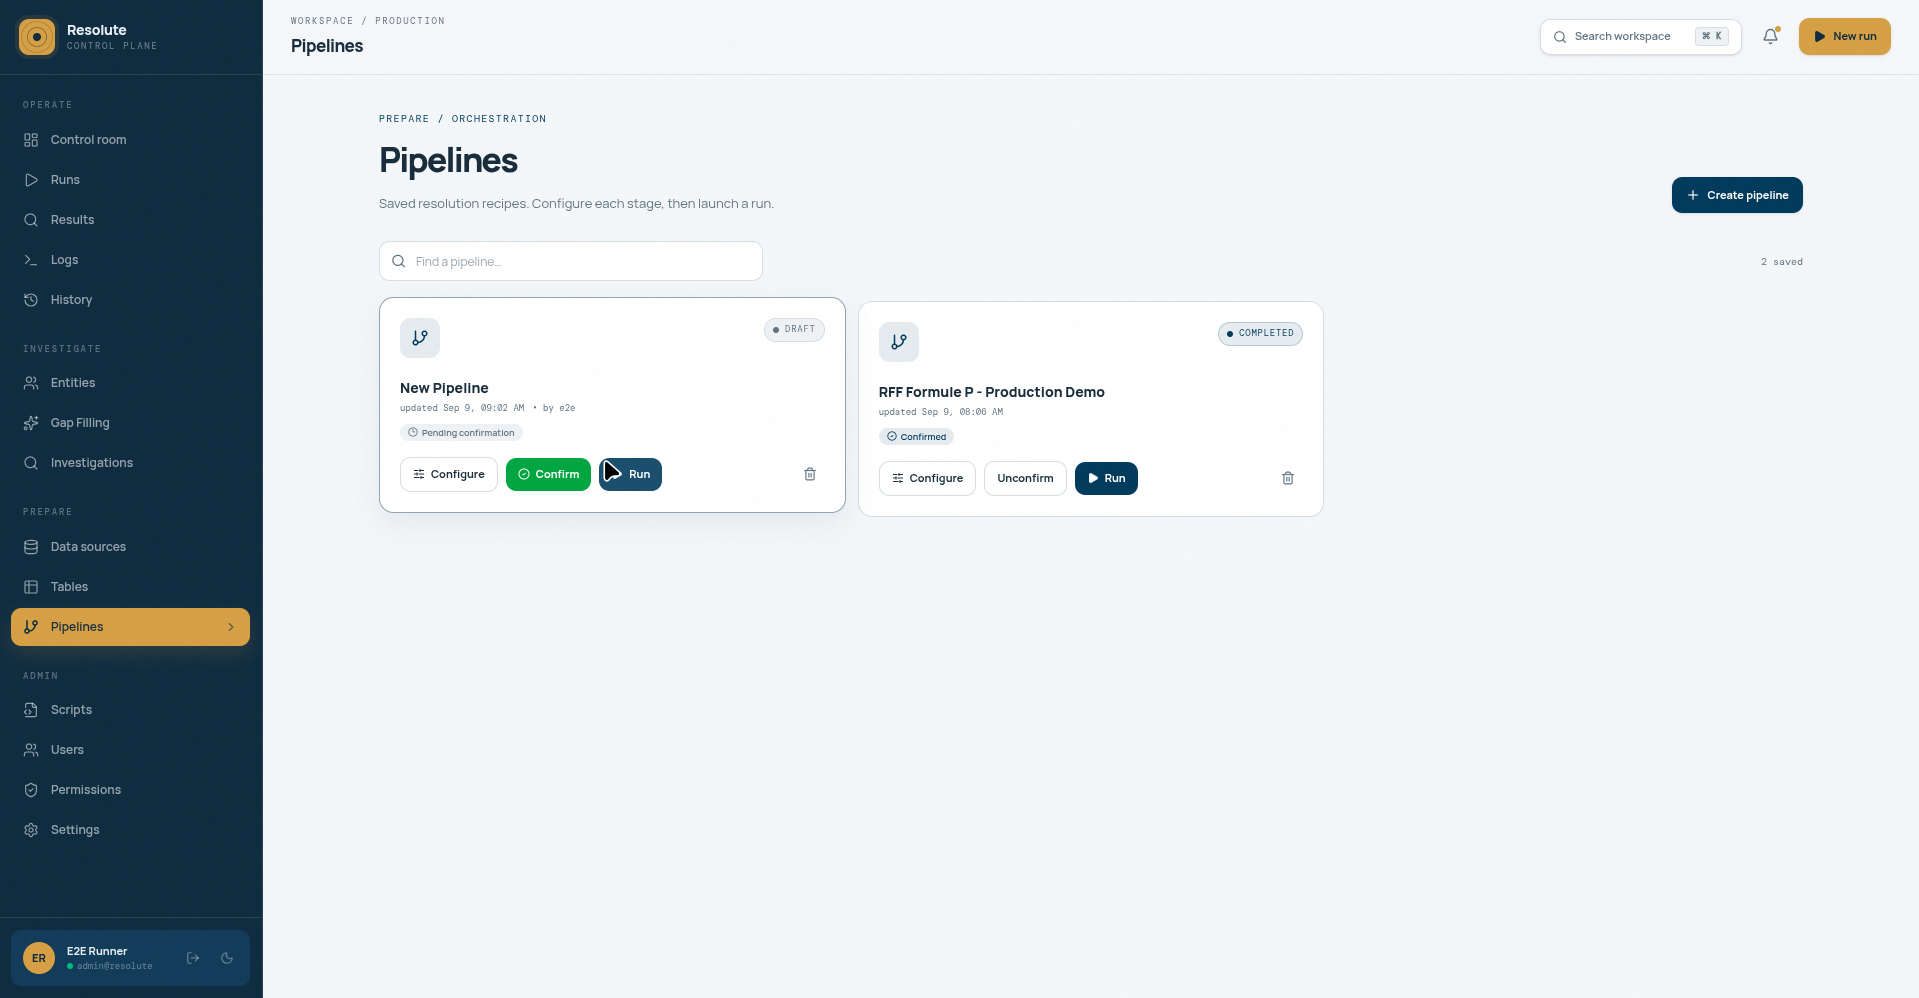
\includegraphics[width=0.9\textwidth]{images/screenshots/pipelines_page.png}
\caption{Page des pipelines : liste des pipelines configurés avec leur état et leurs actions disponibles.}
\label{fig:shot-pipelines}
\end{figure}

\begin{figure}[H]
\centering
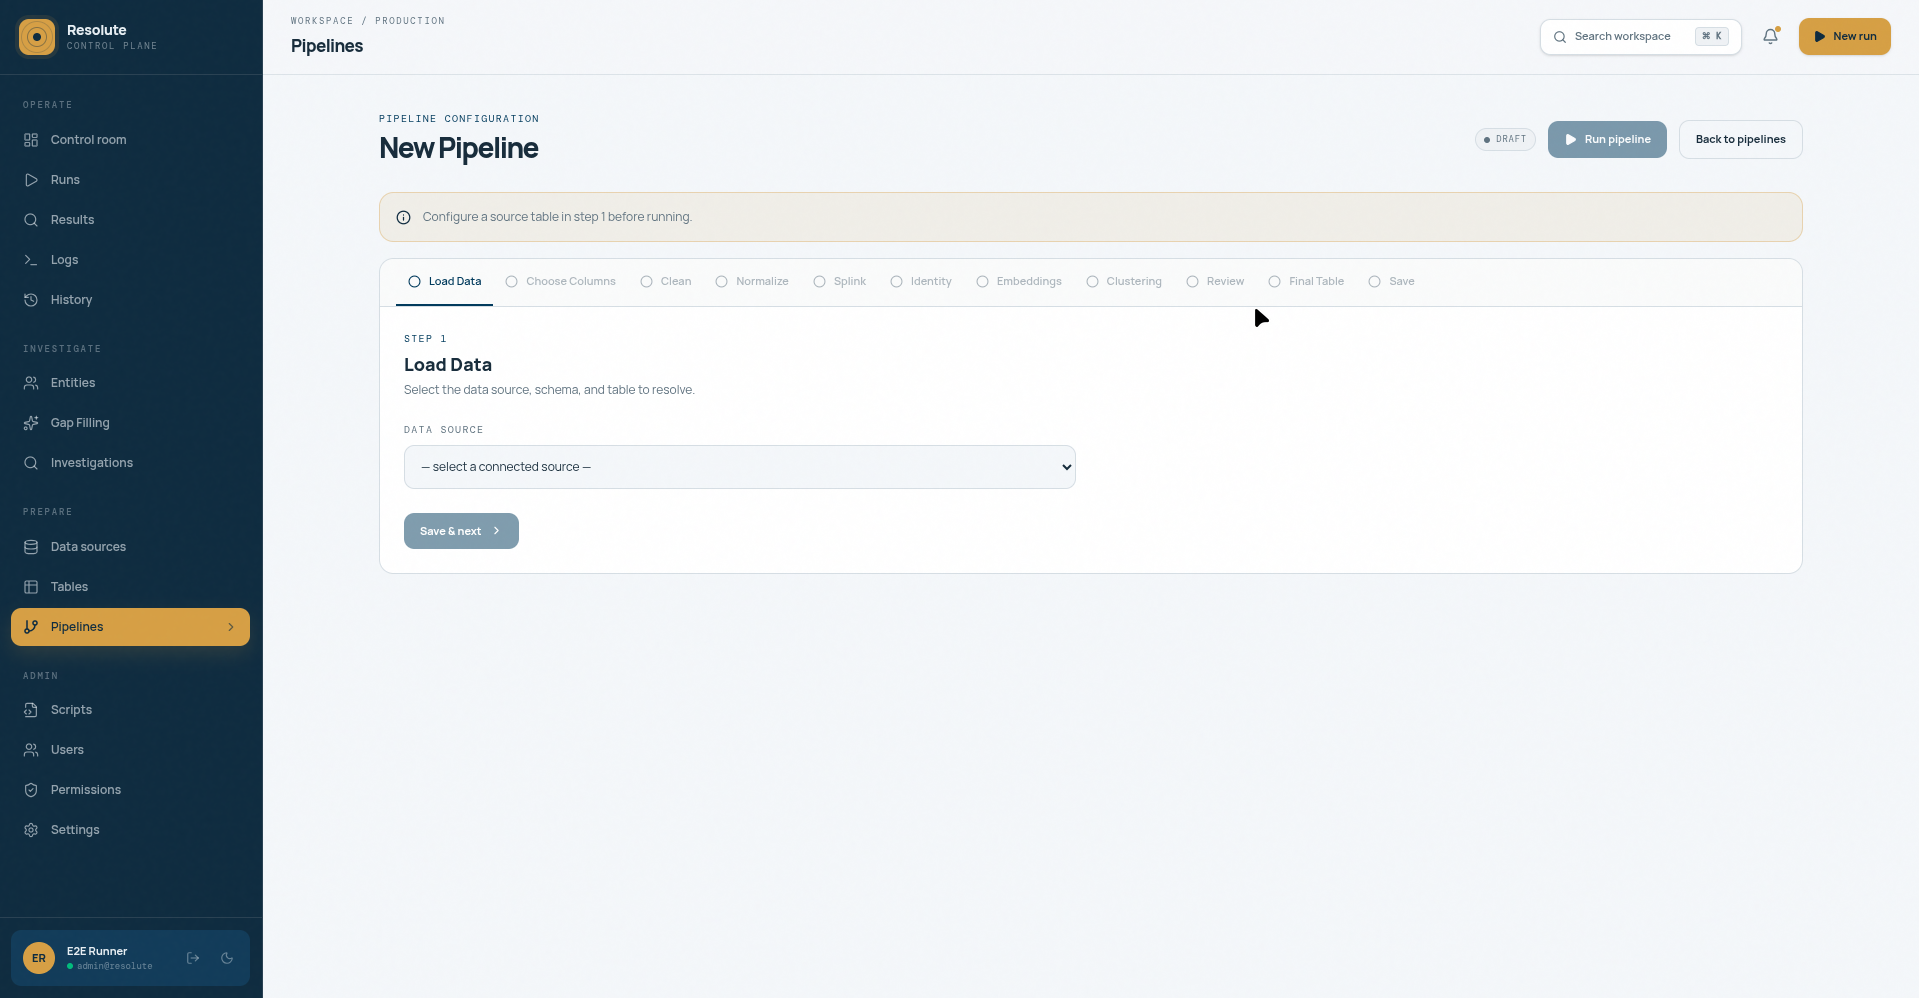
\includegraphics[width=0.9\textwidth]{images/screenshots/pipeline_creation.png}
\caption{Écran de création d'un pipeline : sélection de la source, de la table et des colonnes à traiter.}
\label{fig:shot-creation}
\end{figure}

\subsection{Suivi des exécutions}

Chaque exécution dispose d'une page de détail qui présente son statut global, la progression étape par étape avec les durées et les volumes traités, les métriques produites par Splink telles que le nombre de paires candidates et retenues, et les journaux d'événements émis par le worker. En cas d'échec, le message d'erreur et l'étape concernée sont mis en évidence pour faciliter le diagnostic.

\begin{figure}[H]
\centering
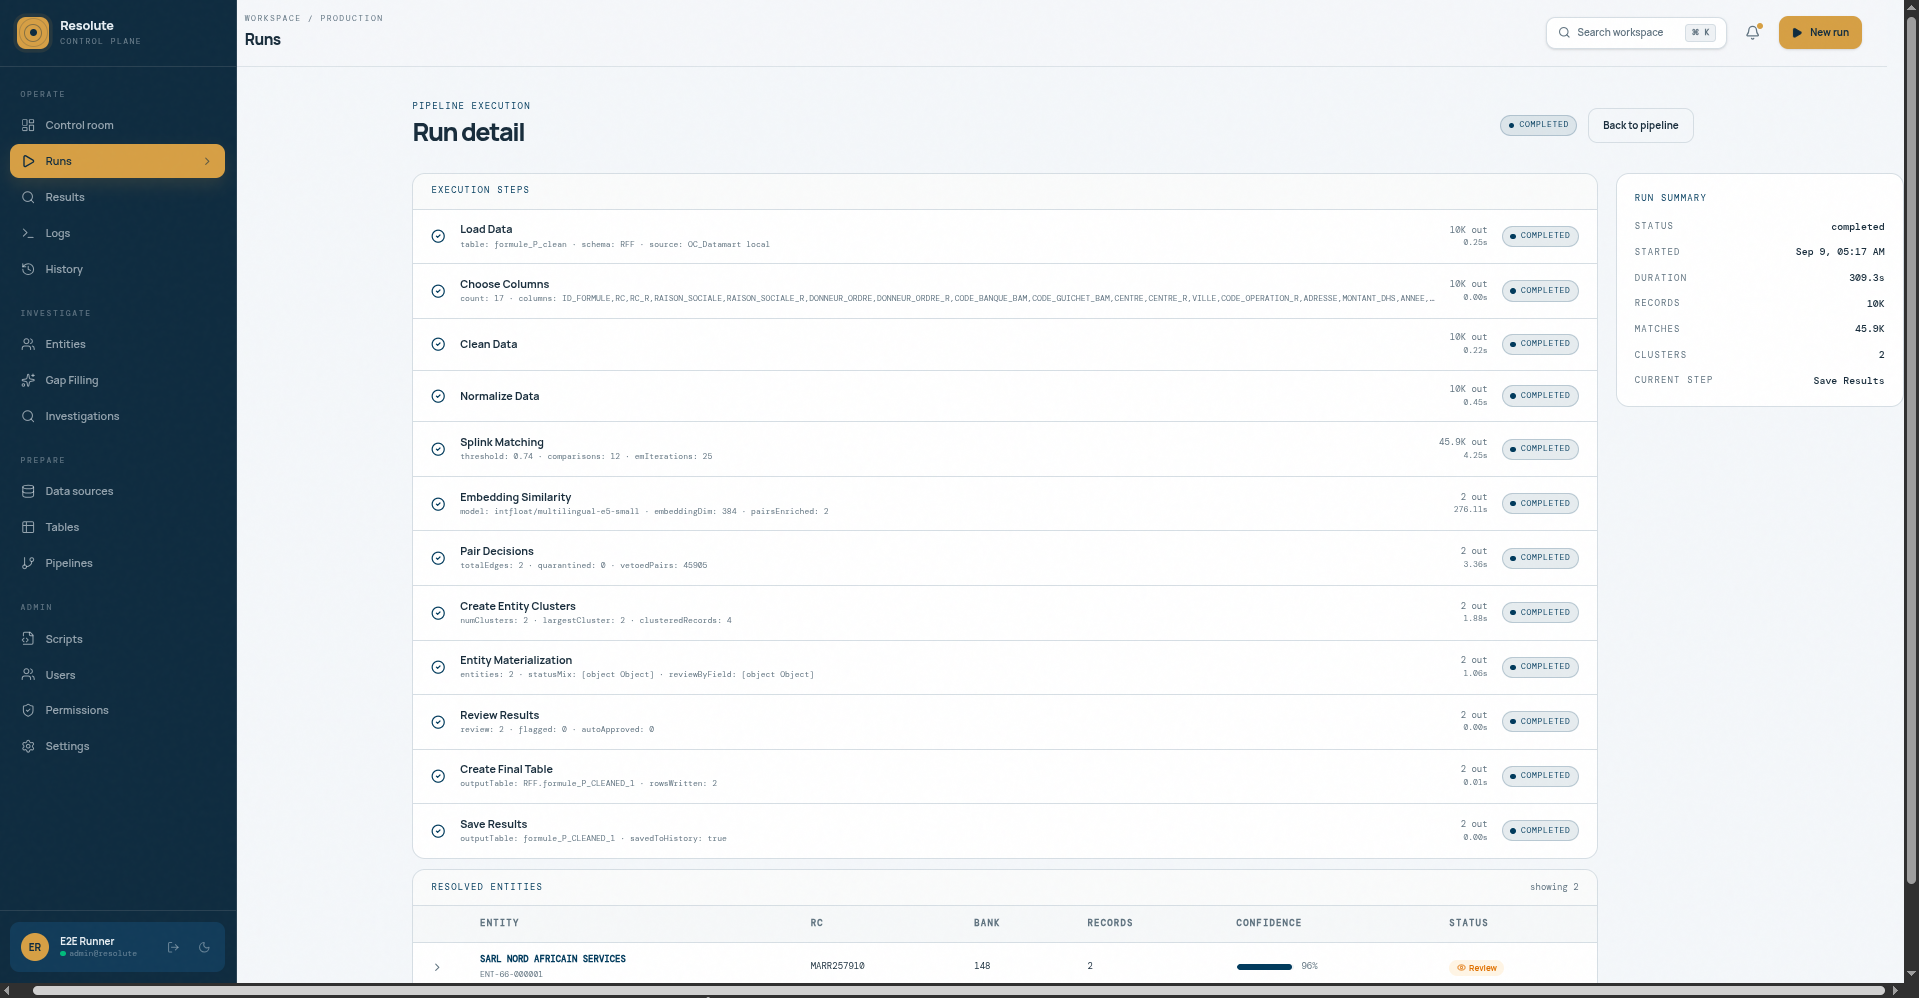
\includegraphics[width=0.9\textwidth]{images/screenshots/pipeline_execution.png}
\caption{Suivi d'une exécution de pipeline : avancement étape par étape avec les volumes traités.}
\label{fig:shot-execution}
\end{figure}

\subsection{Visualisation des entités}

La page des entités présente la liste des opérateurs identifiés par le pipeline. Chaque ligne affiche l'identifiant de l'entité, son nom canonique, ses codes de banque et de guichet, le nombre de déclarations qui lui sont rattachées et son statut. Le statut est matérialisé par un code couleur : les entités de confiance élevée sont approuvées automatiquement, les entités de confiance intermédiaire sont proposées à la révision, et les entités de faible confiance ou de taille anormale sont signalées. La fiche détaillée d'une entité présente l'ensemble de ses déclarations avec leurs champs, en distinguant les versions déclarées et corrigées des identifiants.

\begin{figure}[H]
\centering
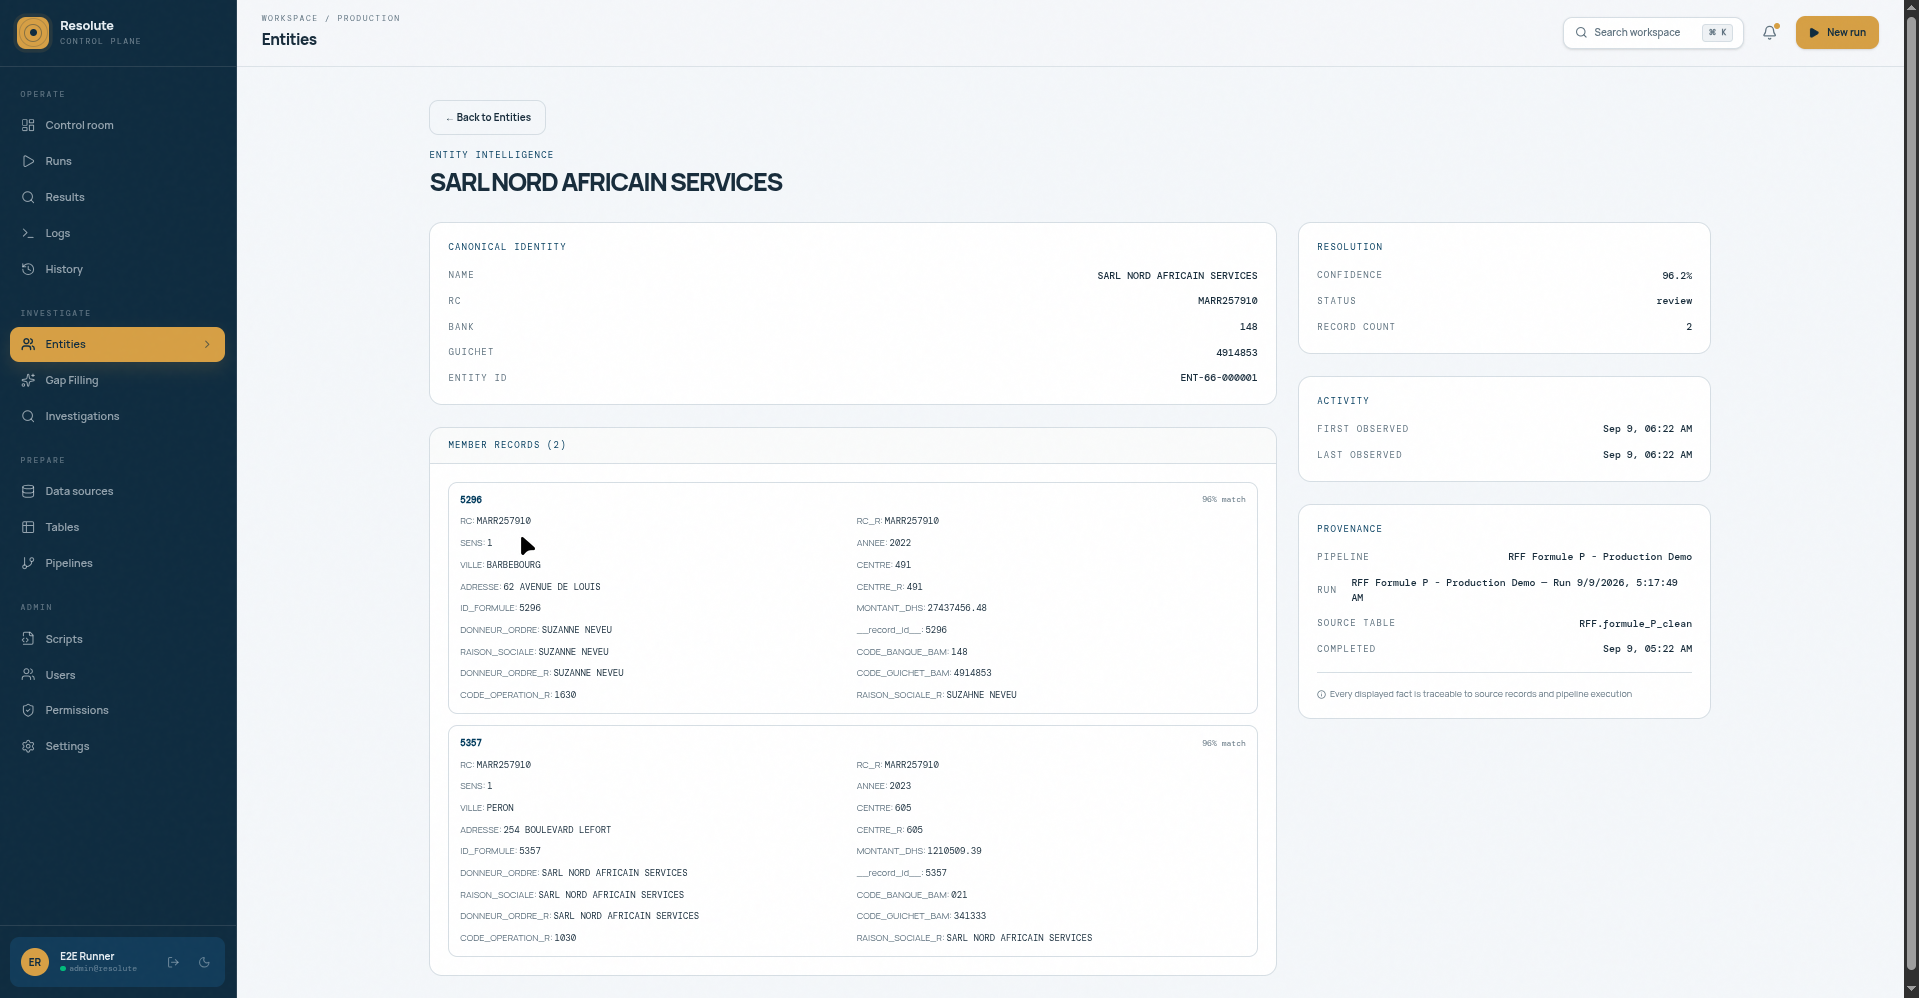
\includegraphics[width=0.9\textwidth]{images/screenshots/entity_details.png}
\caption{Fiche détaillée d'une entité : attributs canoniques et déclarations rattachées avec leurs champs.}
\label{fig:shot-entite}
\end{figure}

\subsection{Recherche intelligente d'opérateurs}

La barre de recherche constitue l'interface principale pour retrouver un opérateur. Elle accepte une requête unique en langage libre et détecte automatiquement le type de recherche : une requête purement numérique est interprétée comme un code de banque, une requête mixte comme un code de guichet, une requête au format du Registre de Commerce comme un identifiant, et toute autre requête comme un nom d'entreprise. La recherche combine l'indexation plein texte de la base avec des filtrages ciblés, en priorisant le nom canonique des entités puis les identifiants exacts. Un moteur de synonymes enrichit la requête avec les variantes connues, les résultats sont dédupliqués par entité, et le tri reflète la pertinence globale. Cette recherche permet ainsi de retrouver un opérateur même lorsque la requête ne reprend exactement aucune des formes stockées en base.

\section*{Conclusion}

Ce chapitre a présenté la transformation du pipeline en une plateforme opérationnelle : une architecture en couches séparées qui isole l'interface, la logique métier et le calcul ; un serveur d'API qui sécurise les accès et persiste l'état du système ; un worker qui exécute les traitements lourds avec un suivi temps réel ; et une interface qui rend l'ensemble accessible à des utilisateurs non informaticiens, de la configuration jusqu'à la recherche d'opérateurs. Le chapitre suivant évalue rigoureusement la qualité des résultats produits par cet ensemble.

\chapter{Évaluation Expérimentale, Résultats et Perspectives}

Les chapitres précédents ont présenté la problématique, la méthodologie et la plateforme. Ce dernier chapitre évalue rigoureusement la solution développée : il décrit le protocole d'évaluation fondé sur un jeu de données synthétique avec vérité terrain, présente les résultats obtenus et les analyses qui les éclairent, rapporte la validation manuelle effectuée sur des cas représentatifs, et discute les limites du travail ainsi que ses perspectives.

\section{Protocole d'évaluation}

\subsection{La nécessité d'une vérité terrain}

Évaluer un système d'Entity Resolution exige de connaître, pour un ensemble de paires d'enregistrements, lesquelles correspondent réellement à une même entité. Sur les données réelles de l'institution, cette vérité terrain n'existe pas : elle nécessiterait l'annotation manuelle de milliers de paires par des experts métier, ce qui représente un effort considérable. Pour cette raison, l'évaluation repose sur un jeu de données synthétique dont la structure reproduit fidèlement celle de la table formule\_P, avec l'avantage décisif que l'entité réelle de chaque enregistrement est connue par construction.

\subsection{Construction du jeu de données synthétique}

Le jeu de données comprend cent mille déclarations réparties entre dix mille opérateurs, chaque opérateur étant représenté par un nombre variable de déclarations. Les champs générés reprennent les colonnes utilisées par le pipeline : identifiants de Registre de Commerce et leurs versions corrigées, raisons sociales déclarées et corrigées, donneur d'ordre, codes de banque et de guichet, ainsi que des champs contextuels tels que la ville et le centre.

Les variations introduites dans les données reproduisent de manière générale les phénomènes observés dans la base réelle : erreurs de frappe par substitution, insertion ou suppression de caractères ; formats hétérogènes d'un même identifiant selon l'émetteur de la déclaration ; champs laissés sans valeur sur certaines lignes ; noms d'entreprises abrégés, tronqués ou formulés différemment ; coexistence de versions déclarées et corrigées parfois divergentes. Le jeu comprend également des opérateurs proches mais distincts, destinés à vérifier que le système ne fusionne pas des entités différentes sous prétexte de leur ressemblance. La correspondance entre chaque enregistrement et son opérateur réel est conservée dans un fichier de référence qui n'est utilisé qu'au moment de l'évaluation, jamais pendant l'exécution du pipeline.

\subsection{Métriques d'évaluation}

L'évaluation utilise les métriques classiques de la classification. La précision mesure la proportion de paires correctement appariées parmi l'ensemble des paires retenues par le système : elle reflète la prudence du système. Le rappel mesure la proportion de paires réellement appariées que le système a su retrouver : il reflète son exhaustivité. Le F-score est la moyenne harmonique de la précision et du rappel, et constitue la mesure synthétique principale car elle pénalise les systèmes qui sacrifieraient entièrement l'une des deux dimensions au profit de l'autre.

\section{Résultats principaux}

Évalué sur le jeu synthétique complet avec la configuration standard du pipeline, c'est-à-dire l'entraînement EM non supervisé, le seuil de décision fixé à 0,80 et le clustering sur graphe, le système retrouve la quasi-totalité des paires réellement appariées tout en commettant très peu de fusions abusives. Autrement dit, la précision et le rappel atteignent tous deux des niveaux élevés, ce qui autorise un usage opérationnel où seules les entités de confiance intermédiaire nécessitent une révision humaine, les autres pouvant être exploitées directement. Les valeurs exactes des métriques dépendent du paramétrage retenu et de la composition du jeu d'évaluation, et ne sont donc pas présentées ici comme des garanties absolues : l'enseignement principal est la robustesse du comportement sur l'ensemble du jeu, et non un chiffre isolé.

\section{Analyses complémentaires}

\subsection{Le rôle du seuil de décision}

Le seuil appliqué à la probabilité de correspondance constitue le principal levier de réglage entre la précision et le rappel. L'analyse de la distribution des scores montre que les probabilités produites par le modèle sont fortement polarisées : les paires manifestement appariées obtiennent des scores très élevés, les paires manifestement distinctes des scores très faibles, et seule une minorité de paires ambiguës se situe dans la zone intermédiaire. Cette polarisation explique la stabilité des résultats autour du seuil retenu de 0,80 : déplacer légèrement le seuil ne modifie qu'à la marge l'ensemble des paires retenues, car peu de paires se trouvent au voisinage immédiat du seuil. Relever fortement le seuil améliorerait marginalement la précision au prix d'une perte de rappel sur les cas ambigus, tandis que l'abaisser produirait l'effet inverse.

\subsection{L'importance de la normalisation}

Les analyses d'ablation, qui consistent à désactiver un composant du pipeline pour mesurer sa contribution, montrent que la normalisation des champs joue un rôle déterminant. Lorsque les identifiants sont comparés sous leurs formes brutes, les variations de format masquent les ressemblances et le modèle ne peut pas exploiter pleinement les indices disponibles. Après normalisation, les formes superficielles disparaissent et les fonctions de similarité se concentrent sur les différences significatives. Cet effet est particulièrement marqué sur les identifiants numériques sujets aux variations de présentation et sur les noms d'entreprises sujets aux variations de formulation des formes juridiques. La leçon générale est que la qualité de la préparation des données conditionne davantage les performances finales que la sophistication du modèle de scoring.

\subsection{Le blocking comme étape critique}

Le blocking détermine l'ensemble des paires que le modèle aura l'occasion d'examiner, et constitue donc un plafond pour le rappel du système. Une stratégie de blocking trop restrictive élimine définitivement des paires réellement appariées, qu'aucune étape ultérieure ne pourra récupérer. À l'inverse, une stratégie trop large noie le modèle sous des candidats non pertinents et alourdit considérablement le calcul. La stratégie multi-passe retenue équilibre ces deux exigences en combinant des règles strictes qui capturent efficacement les cas évidents et des règles larges qui servent de filet de sécurité pour les cas dégradés. L'expérience confirme que le soin apporté aux règles de blocage est au moins aussi important que le réglage du modèle lui-même.

\subsection{Apport des embeddings neuronaux}

La comparaison entre les approches de similarité textuelle montre un résultat instructif : sur les noms d'entreprises, une représentation classique fondée sur les termes discriminants obtient une précision légèrement supérieure à celle des plongements neuronaux multilingues. Ce résultat s'explique par la nature des données : les noms d'entreprises sont des séquences courtes où quelques termes distinctifs suffisent à discriminer les entités, et où la compréhension fine du sens apporte peu par rapport à la reconnaissance des termes. Les plongements conservent néanmoins un intérêt pour les cas ambigus où les formulations diffèrent profondément tout en désignant la même entreprise, et leur combinaison à parts égales avec le score probabiliste n'altère pas les performances globales. Ils constituent donc un enrichissement utile mais non décisif sur ce type de données.

\subsection{Comparaison des stratégies de clustering}

Les deux stratégies de clustering ont été comparées sur les mêmes paires retenues. Les composantes connexes produisent des groupes complets mais exposés au phénomène d'enchaînement, où un lien faible suffit à fusionner artificiellement deux entités distinctes. L'algorithme de Leiden produit des groupes plus resserrés en ne conservant que les communautés à structure interne forte, au prix d'un temps de calcul légèrement supérieur qui reste néanmoins négligeable devant celui de l'entraînement et de la prédiction. Pour un usage opérationnel où les fusions abusives sont plus coûteuses que les fragmentations résiduelles, la sélectivité de Leiden constitue un avantage.

\subsection{Synthèse qualitative des analyses}

Le tableau suivant résume l'apport observé de chaque composant, sans valeur chiffrée, tel qu'il ressort des analyses d'ablation et des comparaisons menées pendant le projet.

\begin{table}[H]
\centering
\caption{Synthèse qualitative de l'apport de chaque composant du pipeline.}
\renewcommand{\arraystretch}{1.3}
\setlength{\tabcolsep}{3pt}
{\small
\begin{tabular}{|p{3.6cm}|p{10.0cm}|}
\hline
\textbf{Composant} & \textbf{Effet observé} \\
\hline
Normalisation des champs & Amélioration déterminante : les variations de format masquaient les ressemblances avant normalisation \\
\hline
Blocking multi-passe & Plafonne le rappel du système : les règles larges servent de filet de sécurité pour les cas dégradés \\
\hline
Seuil de décision & Comportement stable autour du seuil retenu, car les scores sont fortement polarisés \\
\hline
Embeddings neuronaux & Enrichissement utile pour les cas ambigus, sans effet décisif sur les noms courts et standardisés \\
\hline
Clustering de Leiden & Groupes plus sélectifs que les composantes connexes, préférables quand les fusions abusives sont coûteuses \\
\hline
\end{tabular}
}
\end{table}

\section{Validation manuelle}

\subsection{Protocole de validation}

En complément de l'évaluation quantitative, un échantillon de résultats a été examiné manuellement pour apprécier la qualité des entités produites dans des situations représentatives. Trois catégories de cas ont été considérées : les doublons manifestes, où des enregistrements aux noms quasi identiques doivent être regroupés ; les quasi-doublons trompeurs, où des enregistrements aux noms similaires mais aux identifiants divergents doivent rester séparés ; et les cas limites, où la décision nécessite un jugement attentif sur l'ensemble des indices disponibles.

\subsection{Observations}

Sur les cas manifestes, le système se comporte comme attendu dans la quasi-totalité des situations. Sur les quasi-doublons trompeurs, la combinaison des indices permet généralement de maintenir la séparation des entités distinctes, notamment grâce au poids accordé aux identifiants structurés. Les cas limites restants relèvent principalement de deux situations : les entreprises homonymes, c'est-à-dire des entreprises distinctes qui partagent exactement le même nom et parfois la même activité, que seul un examen des identifiants officiels permet de départager ; et les entreprises existant sous plusieurs formes juridiques successives, où la décision de fusionner ou non dépend d'une connaissance de l'histoire de l'entreprise que les données ne contiennent pas toujours. Ces situations justifient le maintien d'une révision humaine pour les entités de confiance intermédiaire. Le tableau suivant résume les cas examinés et le comportement attendu du système pour chacun.

\begin{table}[H]
\centering
\caption{Cas de validation manuelle et comportement attendu du système.}
\renewcommand{\arraystretch}{1.3}
\setlength{\tabcolsep}{3pt}
{\small
\begin{tabular}{|p{4.5cm}|p{9.1cm}|}
\hline
\textbf{Cas} & \textbf{Comportement attendu} \\
\hline
Doublons manifestes & Regroupement des enregistrements aux noms quasi identiques en une seule entité \\
\hline
Quasi-doublons trompeurs & Maintien de la séparation des entités distinctes malgré la ressemblance des noms \\
\hline
Entreprises homonymes & Révision humaine, car le nom seul ne permet pas de trancher \\
\hline
Formes juridiques successives & Révision humaine, car la décision dépend de l'histoire de l'entreprise \\
\hline
\end{tabular}
}
\end{table}

\section{Limites}

Trois limites principales doivent être signalées :

\begin{itemize}
    \item La nature synthétique des données d'évaluation : aussi fidèle soit la reproduction des phénomènes observés, un jeu synthétique ne capture pas nécessairement toutes les spécificités des données historiques accumulées sur plusieurs années, avec leurs évolutions de format et leurs cas particuliers. Une validation complémentaire sur un échantillon de données réelles annotées manuellement reste donc nécessaire avant tout usage en production.
    \item Le passage à l'échelle : le pipeline a été évalué sur des volumes de l'ordre de la centaine de milliers de déclarations, tandis que la base réelle en contient plusieurs millions. Les étapes les plus coûteuses, à savoir le blocking, l'entraînement EM et la prédiction, devront être testées et éventuellement optimisées sur ces volumes, par exemple par un traitement partitionné ou par une parallélisation accrue.
    \item L'hypothèse d'indépendance conditionnelle des champs sur laquelle repose le modèle probabiliste : en pratique, certains champs sont corrélés entre eux, comme le code de guichet qui dépend de la banque, ou la forme juridique qui fait partie du nom. Cette hypothèse simplificatrice n'empêche pas d'excellentes performances empiriques, mais elle peut biaiser les probabilités estimées dans les cas ambigus.
\end{itemize}

\section{Perspectives}

Les perspectives s'ordonnent en trois horizons. À court terme, la priorité est la validation du pipeline sur un échantillon de données réelles avec revue manuelle des entités par les experts métier de l'institution. Cette validation permettra de confirmer les performances mesurées sur données synthétiques et d'identifier les adaptations nécessaires aux spécificités des données historiques.

À moyen terme, plusieurs enrichissements sont envisageables :

\begin{itemize}
    \item L'optimisation des performances pour le traitement de volumes de plusieurs millions de déclarations.
    \item L'intégration du pipeline dans le processus périodique de chargement des déclarations, afin que les nouvelles déclarations soient rattachées aux entités existantes au fil de l'eau.
    \item Le développement d'un tableau de bord de suivi de la qualité des identifiants, qui alerterait sur les dégradations et orienterait les efforts de fiabilisation à la source.
    \item La mise en place d'un apprentissage actif, où les corrections apportées par les analystes lors de la révision alimenteraient l'amélioration continue du système.
\end{itemize}

À long terme, le périmètre pourrait être étendu à d'autres tables de déclarations, et les entités résolues pourraient être rapprochées des référentiels externes d'entreprises pour enrichir encore la connaissance des opérateurs.

\section*{Conclusion}

Ce chapitre a démontré empiriquement l'efficacité de l'approche retenue : sur un jeu de données représentatif avec vérité terrain, le système retrouve la quasi-totalité des paires réellement appariées tout en commettant très peu de fusions abusives, et ce sans aucune donnée annotée grâce à l'entraînement non supervisé. Les analyses ont éclairé le rôle de chaque composant et confirmé que la préparation des données et le blocking sont au moins aussi déterminants que le modèle de scoring. La validation manuelle a circonscrit les situations qui justifient le maintien d'une révision humaine. Les limites identifiées tracent une feuille de route claire vers un usage en production, dont la première étape est la validation sur données réelles.


%------------- Conclusion Générale ----------------
\chapter*{Conclusion G\'{e}n\'{e}rale}
\label{chapter:Conclusion}
\addcontentsline{toc}{chapter}{Conclusion G\'{e}n\'{e}rale}
\setcounter{section}{0}

\section{Bilan g\'{e}n\'{e}ral}

Au terme de ce projet consacr\'{e} \`{a} l'apport de l'Entity Resolution et du Machine Learning dans l'am\'{e}lioration de la qualit\'{e} des donn\'{e}es des op\'{e}rateurs de change \`{a} l'Office des Changes, plusieurs enseignements fondamentaux ont pu \^{e}tre d\'{e}gag\'{e}s.

Ce rapport a permis, dans un premier temps, de pr\'{e}senter le cadre institutionnel de l'Office des Changes, dont la strat\'{e}gie 2025--2029 place la digitalisation et le contr\^{o}le intelligent parmi ses priorit\'{e}s. Dans un second temps, la m\'{e}thodologie du linkage probabiliste multi-champs a \'{e}t\'{e} expos\'{e}e et justifi\'{e}e, et chaque \'{e}tape du pipeline a \'{e}t\'{e} d\'{e}crite en d\'{e}tail, depuis la pr\'{e}paration des donn\'{e}es jusqu'\`{a} la mat\'{e}rialisation des entit\'{e}s. Dans un troisi\`{e}me temps, l'architecture de la plateforme web a \'{e}t\'{e} pr\'{e}sent\'{e}e, avec la communication entre ses composants et ses fonctionnalit\'{e}s de configuration, de suivi, de visualisation et de recherche. Enfin, l'\'{e}valuation exp\'{e}rimentale sur donn\'{e}es synth\'{e}tiques avec v\'{e}rit\'{e} terrain a valid\'{e} l'efficacit\'{e} de l'ensemble.

\section{R\'{e}ponse \`{a} la probl\'{e}matique}

Le syst\`{e}me d\'{e}velopp\'{e} r\'{e}pond \`{a} la probl\'{e}matique pos\'{e}e \`{a} travers cinq contributions concr\`{e}tes. La premi\`{e}re est un pipeline d'Entity Resolution en neuf \'{e}tapes, o\`{u} chaque \'{e}tape est ind\'{e}pendante, configurable et observable, depuis le chargement des d\'{e}clarations jusqu'\`{a} l'\'{e}criture des entit\'{e}s r\'{e}solues. La deuxi\`{e}me est une pr\'{e}paration des donn\'{e}es en deux couches, qui combine un nettoyage g\'{e}n\'{e}rique et une normalisation m\'{e}tier tenant compte des sp\'{e}cificit\'{e}s marocaines des identifiants. La troisi\`{e}me est un moteur probabiliste fond\'{e} sur Splink avec entra\^{i}nement non supervis\'{e}, enrichi de mani\`{e}re optionnelle par la similarit\'{e} s\'{e}mantique neuronale et compl\'{e}t\'{e} par un clustering sur graphe avec mat\'{e}rialisation d'attributs canoniques. La quatri\`{e}me est une plateforme web compl\`{e}te qui rend l'ensemble accessible \`{a} des utilisateurs non informaticiens et qui propose une recherche intelligente d'op\'{e}rateurs. La cinqui\`{e}me est une \'{e}valuation rigoureuse sur jeu synth\'{e}tique avec v\'{e}rit\'{e} terrain, qui \'{e}tablit un F-score de 0,993 et qui \'{e}claire le r\^{o}le de chaque composant par des analyses d'ablation et une validation manuelle.

\section{D\'{e}marche m\'{e}thodologique}

La d\'{e}marche m\'{e}thodologique constitue l'apport le plus durable de ce projet. Elle a montr\'{e} que les approches fond\'{e}es sur un identifiant unique ou sur des comparaisons exactes sont insuffisantes face aux variations et aux valeurs manquantes des donn\'{e}es r\'{e}elles. Elle a \'{e}tabli que la combinaison d'indices faibles par un mod\`{e}le probabiliste permet d'atteindre une qualit\'{e} quasi parfaite sans aucune donn\'{e}e annot\'{e}e. Elle a confirm\'{e} que la pr\'{e}paration des donn\'{e}es et le blocking sont au moins aussi d\'{e}terminants que le mod\`{e}le de scoring lui-m\^{e}me. Et elle a circonscrit avec pr\'{e}cision les situations qui justifient le maintien d'un contr\^{o}le humain, plut\^{o}t que de pr\'{e}tendre \`{a} une automatisation totale.

\section{Limites et perspectives}

L'absence de validation sur donn\'{e}es r\'{e}elles constitue la principale limite actuelle : seule une revue manuelle d'un \'{e}chantillon r\'{e}el par les experts m\'{e}tier permettra de confirmer les performances mesur\'{e}es sur donn\'{e}es synth\'{e}tiques. Le passage \`{a} l'\'{e}chelle vers des volumes de plusieurs millions de d\'{e}clarations devra \^{e}tre test\'{e} et optimis\'{e}. L'hypoth\`{e}se d'ind\'{e}pendance des champs, bien que sans cons\'{e}quence empirique majeure, invite \`{a} la prudence dans l'interpr\'{e}tation des probabilit\'{e}s individuelles.

Les perspectives s'ordonnent naturellement : validation sur donn\'{e}es r\'{e}elles \`{a} court terme, int\'{e}gration dans le processus p\'{e}riodique de chargement et tableau de bord de qualit\'{e} \`{a} moyen terme, extension \`{a} d'autres tables et rapprochement avec des r\'{e}f\'{e}rentiels externes \`{a} long terme.

\bigskip
\noindent En d\'{e}finitive, ce projet aura permis de d\'{e}montrer qu'une probl\'{e}matique de qualit\'{e} des donn\'{e}es peut \^{e}tre adress\'{e}e par une approche technique rigoureuse combinant pr\'{e}paration des donn\'{e}es, Entity Resolution probabiliste et clustering non supervis\'{e}, le tout int\'{e}gr\'{e} dans une plateforme op\'{e}rationnelle et valid\'{e} par une \'{e}valuation rigoureuse. La plateforme est fonctionnelle, l'architecture est extensible, la m\'{e}thodologie est reproductible et les r\'{e}sultats sont \'{e}tablis.


\nocite{*}
\bibliographystyle{ieeetr}
\bibliography{bibliography}
\end{document}
